\documentclass[10pt,journal,comsoc,final]{IEEEtran}

%\usepackage[latin1]{inputenc}
\usepackage{graphicx}
\usepackage{algpseudocode}
\usepackage{algorithm}
\usepackage[english]{babel}
\usepackage{amssymb}
%\usepackage{amsmath}
\usepackage{mathtools}
\usepackage{subfigure}
%\usepackage[space]{cite}
\usepackage{xcolor}
\usepackage{bm}
%\usepackage{multirow}
%\usepackage[scaled]{helvet}
\usepackage{cite}
%\usepackage[utf8]{inputenc}
%\usepackage{wallpaper}

\newtheorem{remark}{Remark}
\newtheorem{lemma}{Lemma}
\DeclareMathOperator{\Tr}{Tr}

\algnewcommand{\LineComment}[1]{\State \(\triangleright\) #1}
\newcommand\ddfrac[2]{\frac{\displaystyle #1}{\displaystyle #2}}

\hyphenation{op-tical net-works semi-conduc-tor}

\begin{document}
\IEEEoverridecommandlockouts

\title{Channel Estimation for Massive MIMO Systems with Pilot Contamination in Multipath Fading Environments}

\author{
\IEEEauthorblockN{Felipe A. P. de Figueiredo\IEEEauthorrefmark{1}, Fabbryccio A. C. M. Cardoso\IEEEauthorrefmark{2} and Gustavo Fraidenraich\IEEEauthorrefmark{3}} \\
\IEEEauthorblockA{\IEEEauthorrefmark{1}Department of Information Technology, Ghent University, Belgium.} \\
\IEEEauthorblockA{\IEEEauthorrefmark{2}CPqD -- Research and Development Center on Telecommunications, Brazil.} \\
\IEEEauthorblockA{\IEEEauthorrefmark{3}DECOM/FEEC -- State University of Campinas (UNICAMP), Brazil.} \\
\IEEEauthorblockA{Email: \IEEEauthorrefmark{1}felipe.pereira@ugent.be, \IEEEauthorrefmark{2}fcardoso@cpqd.com.br, \IEEEauthorrefmark{3}gf@decom.fee.unicamp.br }
}

\maketitle

\begin{abstract}
Massive MIMO is a promising technology which provides better performance in terms of data rate and link reliability. Although promising, each base station (BS) needs accurate estimation of the various channels in order to achieve the benefits offered by Massive MIMO. Therefore, channel estimation is of crucial importance for systems employing such technology. In particular, channel estimation in multipath fading environments suffering from pilot contamination poses a great challenge to such systems. In this work, we introduce a simple and practical channel estimator for multipath multi-cell massive MIMO TDD systems with pilot contamination. Least squares (LS) channel estimators present low performance under moderate to strong pilot contamination, while minimum mean square error (MMSE) estimators perform much better than LS estimators in such conditions. However, MMSE estimators present an issue that prevents its adoption in practical systems, namely the assumption that there is perfect knowledge of the cross-cell large scale coefficients. The proposed estimator does not present any of the issues mentioned above and additionally, provides performance that improves as the number of paths of the channels increases, approaching that of the MMSE estimator. An approximate analytical mean square error (MSE) expression is also derived for the proposed estimator.
\end{abstract}

\begin{IEEEkeywords}
Massive MU-MIMO, channel estimation, pilot contamination, multipath, Zadoff-Chu sequences.
\end{IEEEkeywords}

%*******************************************INTRODUCTION*********************************************
\section{Introduction}
%***************************************************************************************************
\IEEEPARstart{L}{arge-Scale Antenna Systems}, also known as Massive MIMO, provide cellular networks with extremely high gains in both, spectral and radiated energy efficiency. The higher spectral efficiency is attained by serving several users simultaneously through spatial multiplexing and the increase in energy efficiency is mostly due to the array gain provided by the large set of antennas \cite{marzetta:noncooperative, larsson:mmimo_next_gen}. 

The improved spectral and radiated energy performances are based on the important assumption that all channels between the transmit and receive antennas are accurately known. Therefore, faithful channel estimation is of fundamental importance to communications systems. Without optimum channel estimation such systems can not attain its expected performance. For cellular communications systems employing Massive MIMO technology, channel estimation is of utmost importance once both precoding and decoding strongly depend on optimum channel estimation. In such systems, the reuse of frequencies by other cells causes interference in channel estimation, degrading it. This problem is known in the literature as pilot contamination \cite{marzetta:noncooperative, marzetta:pilotContamination}.

Canonical Massive MIMO systems operate in time division duplex (TDD) mode, where uplink and downlink transmissions take place in the same frequency resource but are separated in time. Some of the reasons to operate in TDD mode are channel reciprocity, pilot overhead cost proportional to the number of terminals and improved estimation quality due to the large number of antennas \cite{marzetta:pilotContamination, emil:10_myths, marzetta:book}. In TDD mode, users transmit pilots in the uplink and a BS estimates the channels normally based on least squares (LS) \cite{Gesbert:coordinated} or minimum mean square error (MMSE) \cite{Debbah:howmanyantennas, Marzetta:finitedimensionalchannels} methods. In the great majority of works out there inter and intracell large-scale fading coefficients are assumed to be perfectly known when applying the MMSE method \cite{Ashikhmi:interference_reduction}.

A myriad of works in the literature tackles the problem of channel estimation only for flat fading channels  \cite{marzetta:pilotContamination, marzetta:book, khushboo:semi_blind_est, tadashi:asynch_mu_chann_est, fang:low_rank, mojtaba:traning_for_decorr_chann_est, Debbah:howmanyantennas, Marzetta:finitedimensionalchannels,Ashikhmi:interference_reduction,Bjornson:LowComplexityPolynomial, Gesbert:coordinated, noh:Pilot_beam_pattern, Truong:Channel_Aging, Muller:Blind_Decontamination, Amin:channelEstPilotCont}, which sometimes does not reflect the true nature of communications channels in practice. Given the extensive number of works in flat-fading channel estimation for massive MIMO TDD systems, the main contribution of the current work is in understanding multipath multi-cell massive MIMO TDD systems with channel training. Specifically, the main contribution is to demonstrate the pilot contamination problem associated with uplink training in multipath fading channels, understand its impact on the operation of multi-cell massive MIMO TDD cellular systems, propose and assess a simple and practical channel estimator to mitigate such problem. 

The present work analyses the performance of some linear estimators and proposes an efficient and practical one that does not require knowledge of inter-cell large-scale fading coefficients for the case when the wireless communication channels present multipath fading behavior, $i.e.$, frequency-selective fading. It is an extension of the work presented in \cite{Amin:channelEstPilotCont} to multipath fading channels. The proposed approach instead of individually estimating the large-scale coefficients estimates a parameter that is the sum of them plus a normalized noise variance. That parameter is substituted back into the MMSE estimator to create the proposed one. We also derive an approximate analytical MSE expression of the proposed estimator. Simulation results show that the performance of the proposed channel estimation method approaches that of the ideal MMSE estimator asymptotically, $i.e.$, $M \to \infty$.

This work is divided into four parts: First, we present the signal model adopted for this study and briefly discuss the LS and MMSE linear estimators. Then, we introduce the proposed channel estimator for multipath channels. Next, some numerical results are presented in order to support the effectiveness of the proposed estimator against the well-known linear estimators. Finally, we present our conclusions. 

%**********************************************SECTION**********************************************
\section{Signal Model}
%***************************************************************************************************
In this work we consider a multi-cell multi-user massive MIMO system employing TDD protocol with $L$ cells where each cell has a BS with $M$ co-located  antennas and $K$ randomly located single antenna users, where $M \gg K$. All the $K$ users in a cell are served at the same time/frequency resource. Fig. \ref{fig:problem_definition} illustrates the problem we are dealing with.

%------------------------------------------------------------------------------
\begin{figure}[b]
\centering
\vspace{-4mm}
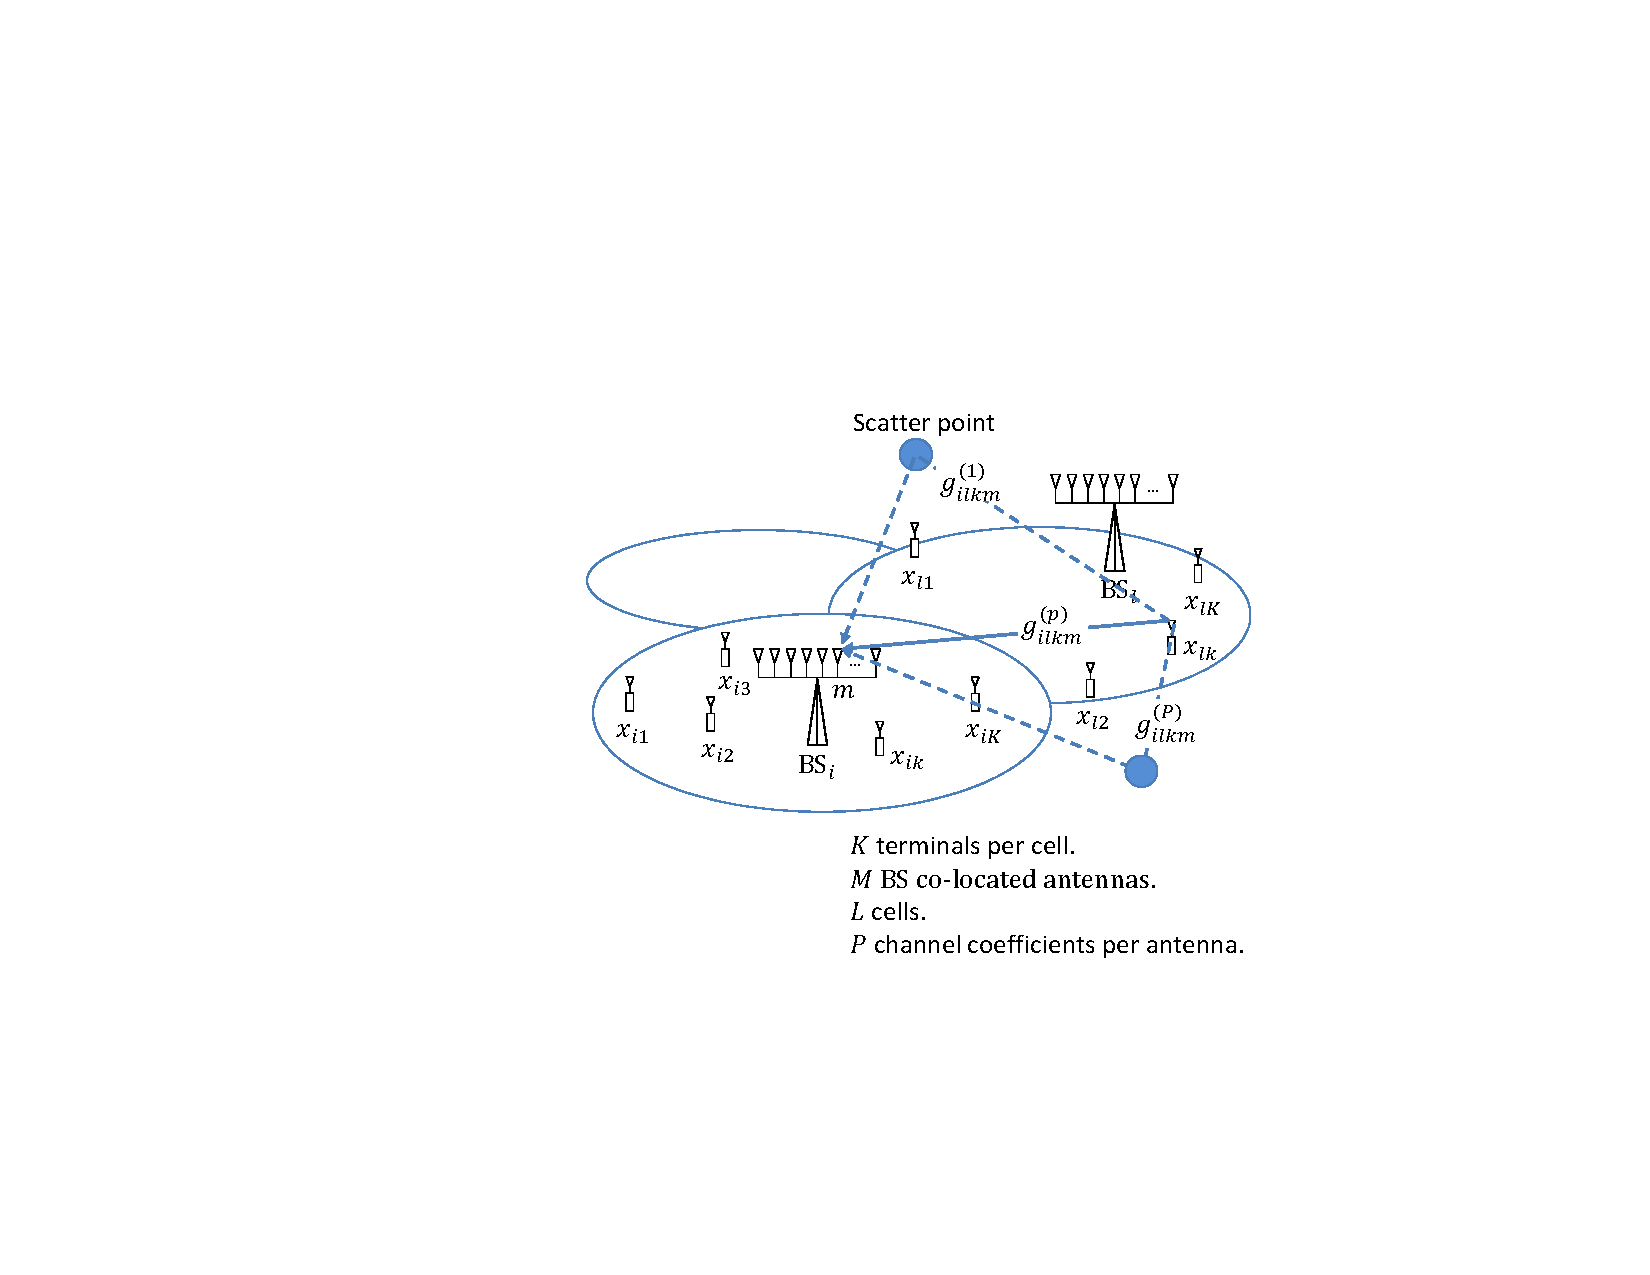
\includegraphics[trim = 0mm 0mm 0mm 0mm, clip=true, scale=0.63]{cropped_problem_definition.pdf}
\caption{Problem definition.}
\label{fig:problem_definition}
\end{figure}
%------------------------------------------------------------------------------

Based on the assumption of channel reciprocity, we adopt the TDD protocol depicted in Fig. \ref{fig:tdd_protocol} and proposed in \cite{marzetta:how_much_training}. Due to the reciprocity principle, only the uplink channels need to be estimated while the downlink channels are equal to the transpose of the uplink channels. It is important to note that the length of the TDD frames is limited by the channel coherence time \cite{marzetta:how_much_training, caire:achivable_dl_rates}. According to the TDD protocol, first, all users in all cells send their uplink training sequences synchronously. After that, the BSs use the training sequences to estimate the uplink channels. Next, the users send uplink data signals. Then, the BSs use the estimated channels to detect uplink data and generate precoding matrices used to transmit downlink data.

%------------------------------------------------------------------------------
\begin{figure}[t]
\centering
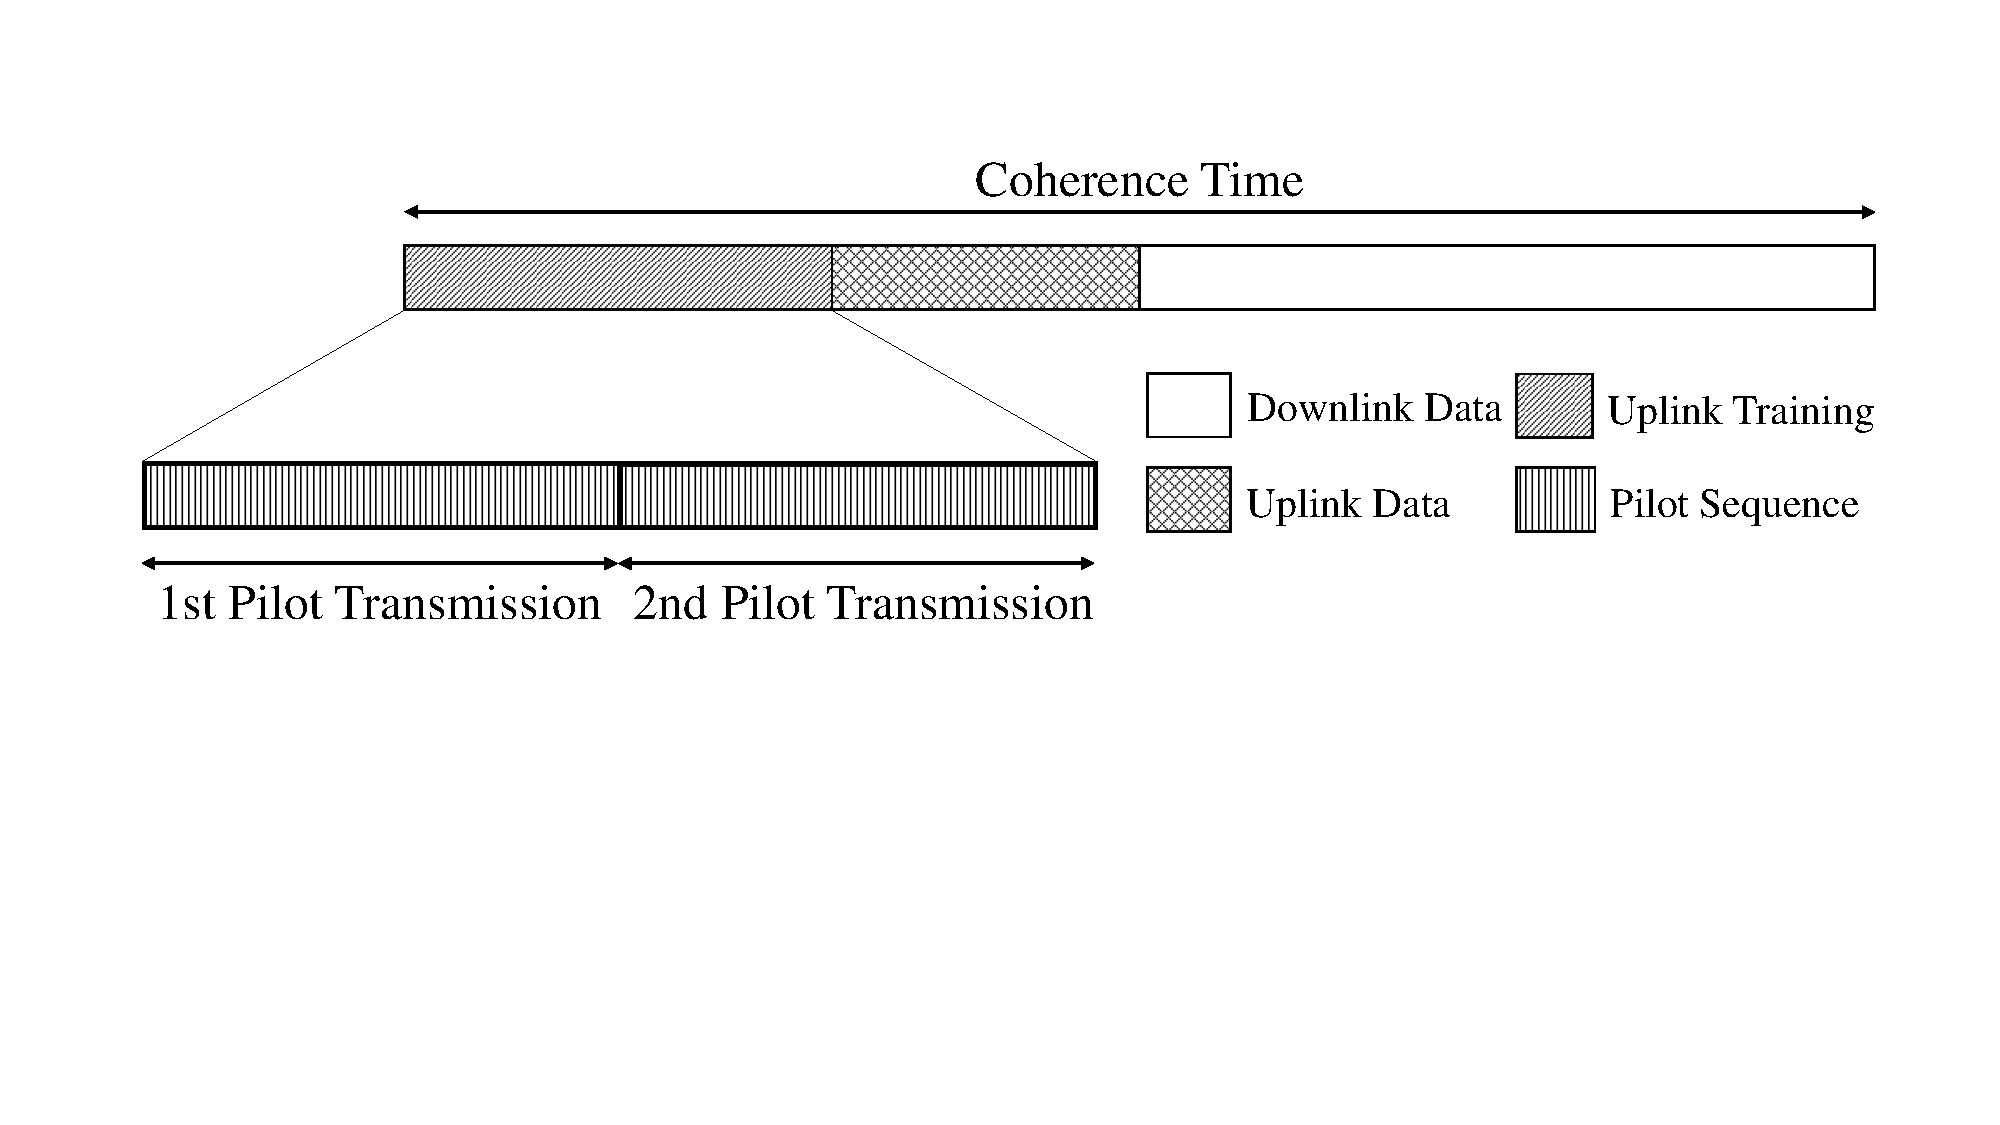
\includegraphics[trim = 0mm 1mm 0mm 0mm, clip=true, scale=0.3]{cropped_TDD_Protocol_Frame_Structure_v2.pdf}
\caption{TDD transmission protocol.}
\label{fig:tdd_protocol}
\vspace{-6mm}
\end{figure}
%------------------------------------------------------------------------------

We also assume in this work wireless radio channels that take into account both large and small scale effects. Large-scale fading represents shadowing and attenuation or path-loss over a large area while small-scale fading refers to the abrupt changes in signal amplitude and phase as a result of very small changes (in the order of $\lambda$/2) in the spatial separation between the user and the BS \cite{rappaport:wireless_comm}. We consider that multipath propagation is the main effect behind small scale fading. Multipath causes multiple copies of a signal to travel over different paths with different propagation delays. These copies are received at the receiver at different phase angles and strengths \cite{sklar:rayleigh_channels}.

The wireless channels are considered static during the channel coherence time and independent across users and antennas. Let $g_{ilkm}^{(p)}$ represent the complex gain of the $p$th path of the channel from user $k$ in cell $l$ to the antenna $m$ of the BS in cell $i$. Additionally, the complex gain $g_{ilkm}^{(p)}$ can be expressed as a complex fast fading factor (small-scale fading) times an amplitude factor that accounts for path-loss and log-normal shadow fading (large-scale fading),
%-----------------------------------------------------------------------------------------
\begin{equation}
\begin{split}
g_{ilkm}^{(p)} = h_{ilkm}^{(p)}\sqrt{\beta_{ilk}}, 
\\ i = 1, \cdots L, \ l = 1, \cdots, L, 
\\ k = 1, \cdots, K, \ m = 1, \cdots, M,
\end{split}
\end{equation}
%-----------------------------------------------------------------------------------------
where the fast fading coefficients, $h_{ilkm}^{(p)}$, are assumed to follow a circularly-symmetric complex normal distribution with $\mathcal{CN}(0,1)$ and the amplitude factor, $\sqrt{\beta_{ilk}}$, is assumed constant with respect to the index of the base station
antenna since the path-loss and shadow fading change slowly
over space \cite{marzetta:noncooperative},  \cite{sklar:rayleigh_channels,tranter:principles}. 

The multipath channels are modeled as $1 \times P$ vectors, $\textbf{g}_{ilkm} = \left[ g_{ilkm}^{(0)}, g_{ilkm}^{(1)}, ..., g_{ilkm}^{(P-1)} \right]$ where $P$ denotes the number of paths of the channel. The overall $M \times KP$ channel matrix is denoted by $\textbf{G}_{il}$ as showed below in \eqref{eq:channel_matrix}. Each column of $\textbf{G}_{il}$ is denoted by $\textbf{G}_{ilk}$ and represents the channels from the $k$th user to the $M$ antennas at the $i$th BS in the $l$th cell. For detection and precoding, BS $i$ needs to know the channels of the users in cell $i$, namely $\{ \textbf{G}_{iik} : \forall k \}$.
%-----------------------------------------------------------------------------------------
\begin{equation}\label{eq:channel_matrix}
\begin{split}
\textbf{G}_{il} = \left[\begin{array}{cccc}
\textbf{g}_{il11} & \textbf{g}_{il21} & \cdots & \textbf{g}_{ilK1} \\
\textbf{g}_{il12} & \textbf{g}_{il22} & \cdots & \textbf{g}_{ilK2} \\
\textbf{g}_{il13} & \textbf{g}_{il23} & \cdots & \textbf{g}_{ilK3} \\
\vdots & \vdots & \ddots & \vdots \\
\textbf{g}_{il1M} & \textbf{g}_{il2M} & \cdots & \textbf{g}_{ilKM} \\ \end{array} \right] \\ = \left[\begin{array}{cccc}
\textbf{G}_{il1} & \textbf{G}_{il2} & \cdots & \textbf{G}_{ilK} \end{array} \right] \hspace{10pt} \\ = \left[\begin{array}{cccc}
\beta_{il1}\textbf{H}_{il1} & \beta_{il2}\textbf{H}_{il2} & \cdots & \beta_{ilK}\textbf{H}_{ilK} \end{array} \right].
\end{split}
\end{equation}
%-----------------------------------------------------------------------------------------

As in the literature, we treat $\lbrace \beta_{ilk} \rbrace$ as being deterministic during the channel estimation  \cite{marzetta:noncooperative, Ashikhmi:interference_reduction, Bjornson:LowComplexityPolynomial, Amin:channelEstPilotCont}.

%*******************************************SUB-SECTION*********************************************
\subsection{Uplink Training}
%***************************************************************************************************
Each user transmits an uplink training sequence so that the BS can estimate the $M$ multipath channels from that user to itself. We assume that users in different cells transmit the same set of pilots at the same time/frequency resource (a typical scenario in massive MIMO) and that the pilot reuse factor is one, the worst possible case \cite{marzetta:noncooperative}.

The pilot signals of $K$ users are represented by a $N \times KP$ matrix $\textbf{S}$ of the form $\textbf{S} = \left[ \textbf{S}_{1},  \textbf{S}_{2},  \cdots, \textbf{S}_{K}\right]$, where $N$ is the length of the pilot sequences. As we are dealing with multipath channels, each one of the $K$ uplink training sequences is convoluted with all the $M$ channels. Therefore, in order to express these convolutions in matrix form, we write each one of the pilots as a $N \times P$ matrix with orthogonality property $\textbf{S}_{k}^{H} \textbf{S}_{k} = N\textbf{I}_{p}$, where $ \textbf{S}_{k}$ is of the form
%-----------------------------------------------------------------------------------------
\begin{equation}\label{eq:pilot_matrix}
\begin{split}
\textbf{S}_{k} = \left[\begin{array}{cccc}
{s}_{k}(0) & {s}_{k}(N-1) & \cdots & {s}_{k}(N-P+1) \\
{s}_{k}(1) & {s}_{k}(0) & \cdots & {s}_{k}(N-P+2) \\
{s}_{k}(2) & {s}_{k}(1) & \cdots & {s}_{k}(N-P+3) \\
\vdots & \vdots & \ddots & \vdots \\
{s}_{k}(N-1) & {s}_{k}(N-2) & \cdots & {s}_{k}(N-P+N) \\ \end{array} \right].
\end{split}
\end{equation}
%-----------------------------------------------------------------------------------------

In order to obtain circular matrices as showed in \eqref{eq:channel_matrix}, users must transmit their pilot sequences twice, making it a $2N$ sequence, as showed in Fig. \ref{fig:tdd_protocol}. This is a direct consequence of the orthogonality property mentioned above. The pilots are created by applying cyclic shifts to Zadoff-Chu root sequences with length $N$, where $N$ is a prime number. These sequences exhibit the useful property that cyclically shifted versions of themselves are orthogonal to each other \cite{zadoffchu:zadoffchu}.
We assume that $N > KP$, this assumption must hold true so that all users have valid pilots, $i.e.$, it must be possible to generate orthogonal pilot sequences out of the same Zadoff-Chu root sequence for all users in the cell.

The received uplink training sequences at BS $i$ can be represented as a $M \times N$ matrix defined as
%-----------------------------------------------------------------------------------------
\begin{equation}\label{eq:received_signal}
\textbf{Y}_{i} = \sqrt{q} \sum^{L}_{l=1}{ \textbf{G}_{il} \textbf{S}^{H} + \textbf{N}_{i}},
\end{equation}
%-----------------------------------------------------------------------------------------
where $q$ is the uplink power or transmit signal to noise ratio (TX SNR) and $\textbf{N}_{i}$ is a $M \times N$ noise matrix with independent and identically distributed elements following $\mathcal{CN}(0,1)$.

%*******************************************SUB-SECTION*********************************************
\subsection{LS Channel Estimator}
%***************************************************************************************************

As showed earlier, $\textbf{S}_{k}$ denotes the $k$th pilot matrix of $\textbf{S}$, therefore, for estimation of the channel $\textbf{G}_{ilk}$ at BS $i$, a sufficient statistic is given by 
%-----------------------------------------------------------------------------------------
\begin{equation}\label{eq:ls_estimator}
\textbf{Z}_{ik} = \frac{1}{\sqrt{q}N} \textbf{Y}_{i} \textbf{S}_{k} = \sum_{l=1}^{L}{\textbf{G}_{ilk}} + \frac{\textbf{N}_{i}\textbf{S}_{k}}{\sqrt{q}N}.
\end{equation}
%-----------------------------------------------------------------------------------------
where $\textbf{Z}_{ik}$ is a $M \times P$ matrix with a $\mathcal{CN}(\textbf{0}_{M \times P},M\zeta_{ik}\textbf{I}_{P})$ distribution where
%-----------------------------------------------------------------------------------------
\begin{equation}\label{eq:zeta}
\zeta_{ik} = \sum_{l=1}^{L}{\beta_{ilk}} +  \frac{1}{qN}.
\end{equation}
%-----------------------------------------------------------------------------------------

Additionally, the term corresponding to noise in \eqref{eq:ls_estimator} has a $\mathcal{CN}(\textbf{0}_{M \times P},\frac{M}{qN}\textbf{I}_{P})$ distribution, $i.e.$, a matrix where the elements are circularly-symmetric complex normal random variables.

The least squares estimator is given by \cite{kay:estimationbook} 
%-----------------------------------------------------------------------------------------
\begin{equation}\label{eq:ls}
\hat{\textbf{G}}_{iik}^{\text{LS}} = \textbf{Z}_{ik}.
\end{equation}
%-----------------------------------------------------------------------------------------

The MSE per antenna of the LS estimator is defined as $\eta_{ik}^{\text{\text{LS}}} = \frac{1}{M} \mathbb{E} \{ \lVert  \hat{\textbf{G}}_{iik}^{\text{LS}} - \textbf{G}_{iik} \rVert^{2} \}$ and given by
%-----------------------------------------------------------------------------------------
\begin{equation}\label{eq:mse_ls}
\eta_{ik}^{\text{\text{LS}}} = (\zeta_{ik} - \beta_{iik}) \textbf{I}_{P}.
\end{equation}
%-----------------------------------------------------------------------------------------

As known, the LS estimator has larger MSE than the MMSE estimator, however, it does not need to know the large-scale fading coefficients, $\beta_{ilk}$.

Differently from \cite{Amin:channelEstPilotCont}, the MSE equation for the LS estimator does not result in a scalar value, instead, it results in an identity matrix, $ \textbf{I}_{P}$, which is multiplied by the same MSE found in that work. This result is due to the $P$ coefficients of the multipath channels. When $P = 1$ equation \eqref{eq:mse_mmse} reduces to equation (5) in \cite{Amin:channelEstPilotCont}.

\begin{remark}Due to pilot contamination, as $q \to\infty $, $\eta_{ik}^{\text{LS}} \to \left( \sum_{l=1,l \neq i}^{L}{\beta_{ilk}} \right) \textbf{I}_{P}$. \end{remark}

%*******************************************SUB-SECTION*********************************************
\subsection{MMSE Channel Estimator}
%***************************************************************************************************

The Bayesian MMSE estimator requires knowledge of statistics of parameters to be estimated as well as those of noise and interference. Many massive MIMO works acquire channel knowledge based on MMSE estimation \cite{marzetta:pilotContamination, Marzetta:finitedimensionalchannels}, and they assume perfect knowledge of all large-scale fading coefficients, $i.e.$, $\{\beta_{ilk}, 1 \leq i, l \leq L, 1 \leq k \leq K\}$ which may not be justifiable in practice. With the perfect knowledge of $\{\beta_{ilk}\}$, the ideal MMSE estimator is given by \cite{kay:estimationbook}
%-----------------------------------------------------------------------------------------
\begin{equation}\label{eq:mmse}
\hat{\textbf{G}}_{iik}^{\text{MMSE}} = \frac{\beta_{iik}}{\zeta_{ik}}\textbf{Z}_{ik},
\end{equation}
%-----------------------------------------------------------------------------------------
where $\hat{\textbf{G}}_{iik}^{\text{MMSE}} \sim \mathcal{CN}(\textbf{0}_{M \times P},\frac{M \beta_{iik}^{2}}{\zeta_{ik}}\textbf{I}_{P})$.

The MSE per antenna of the ideal MMSE channel estimator is defined as $\eta_{ik}^{\text{MMSE}} = \frac{1}{M} \mathbb{E} \left\lbrace \lVert  \hat{\textbf{G}}_{iik}^{\text{MMSE}} - \textbf{G}_{iik} \rVert^{2} \right\rbrace$ and given by \cite{kay:estimationbook}
%-----------------------------------------------------------------------------------------
\begin{equation}\label{eq:mse_mmse}
\eta_{ik}^{\text{MMSE}} = \beta_{iik}\left( 1 - \frac{\beta_{iik}}{\zeta_{ik}} \right) \textbf{I}_{P}.
\end{equation}
%-----------------------------------------------------------------------------------------

The MSE per antenna, $\eta_{ik}^{\text{MMSE}}$, decreases with increasing $q$, decreasing $\beta_{iik}$, or decreasing $\beta_{iik}$ (smaller interference level). Again, the MSE per antenna for the MMSE estimator only differs from the findings in \cite{Amin:channelEstPilotCont} by the identity matrix, $ \textbf{I}_{P}$. When $P = 1$ equation \eqref{eq:mse_mmse} reduces to equation (5) in \cite{Amin:channelEstPilotCont}.

\begin{remark} Due to pilot contamination, as $q \to\infty$, $\eta_{ik}^{\text{MMSE}} \to \beta_{iik} \left( 1 - \frac{\beta_{iik}}{\sum_{l=1}^{L}{\beta_{ilk}}} \right) \textbf{I}_{P}$. \end{remark}

%**********************************************SECTION**********************************************
\section{Proposed Channel Estimator}
%***************************************************************************************************

Acquisition of inter-cell large-scale fading coefficients is unjustified due to the excessive overhead necessary to estimate them \cite{fengChen:largeScale}. For instance, in the case where there are $L$ cells with $K$ users in each cell, each one of the Base Stations would need to estimate $(L-1)K$ inter-cell large-scale fading coefficients. Through analysis of the MMSE channel estimator it is possible to notice that instead of individual ${\beta_{ilk}}$ coefficients as assumed in the existing works \cite{marzetta:noncooperative, marzetta:pilotContamination, Debbah:howmanyantennas, Marzetta:finitedimensionalchannels, Ashikhmi:interference_reduction, Bjornson:LowComplexityPolynomial, Gesbert:coordinated}, we only need to know $\zeta_{ik}$. This observation results in a simple but yet efficient solution to the issue of acquisition of the inter-cell large-scale coefficients. Therefore, the approach we put forward in this work consists of the estimation of $\zeta_{ik}$ and its subsequent use in the MMSE estimator \eqref{eq:mmse}, yielding the estimator derived next.

A possible minimum variance unbiased estimator (MVUE) of $\zeta_{ik}$ given the observed signal $\textbf{Z}_{ik}$ is given by \cite{kay:estimationbook}

%-----------------------------------------------------------------------------------------
\begin{equation}\label{eq:mvue}
\hat{\zeta_{ik}} =  \frac{ \Tr \left(  \lVert \textbf{Z}_{ik} \rVert^{2} \right) }{MP}.
\end{equation}
%-----------------------------------------------------------------------------------------

The $\Tr(.)$ operation removes all inner products between estimated channels of the $k$th user to the $M$ antennas at the $i$th BS while summing all elements of the main diagonal. Other possible MVUE's would be the ones that take into account one or more (less than $P$) elements in the main diagonal of $\lVert \textbf{Z}_{ik} \rVert^{2}$. 

Equation \eqref{eq:mvue} arises from the fact that $\mathbb{E} \left\lbrace \lVert \textbf{Z}_{ik} \rVert^{2} \right\rbrace = M \zeta_{ik} \textbf{I}_{P}$, that the unbiased estimator has $\mathbb{E} \{ \hat{\zeta_{ik}} \} =\zeta_{ik}$ and also from the observation that as $P$ increases, the term $ \Tr \left(  \lVert \textbf{Z}_{ik} \rVert^{2} \right) / P$ tends to $M\zeta_{ik}$, therefore resulting in a better estimator in the sense that it approaches $\zeta_{ik}$ faster than the other possible MVUE's once it is the average over all $P$ inner products in the main diagonal of $\lVert \textbf{Z}_{ik} \rVert^{2}$.

It is possible to write $\zeta_{ik} = \hat{\zeta_{ik}} + e_{ik}$ where $e_{ik}$ is the estimation error. Since $\textbf{Z}_{ik} \sim \mathcal{CN}(\textbf{0}_{M \times P},M\zeta_{ik}\textbf{I}_{P})$, $ \hat{\zeta_{ik}}$ has a Gamma distribution with shape ($k$) equal to $PM$, scale ($\theta$) equal to $\zeta_{ik}$, $ \mathbb{E} \{ \hat{\zeta_{ik}} \} = \zeta_{ik}$ and $\text{var}\{ \hat{\zeta_{ik}} \} = \zeta_{ik}^{2}/MP$. Under the MVUE framework, the parameter to be estimated is considered to be deterministic \cite{kay:estimationbook}, and thus $e_{ik}$ has zero mean and variance given by $\zeta_{ik}^{2}/MP$, which is the same variance of $\hat{\zeta_{ik}}$.

Finally, swapping $\zeta_{ik}$ with $\hat{\zeta_{ik}}$ in \eqref{eq:mmse} produces the proposed channel estimator, which is defined by
%-----------------------------------------------------------------------------------------
\begin{equation}\label{eq:proposed}
\hat{\textbf{G}}_{iik}^{\text{prop}} = MP \frac{\beta_{iik}}{ \Tr \left( \lVert \textbf{Z}_{ik} \rVert^{2} \right) }\textbf{Z}_{ik}.
\end{equation}
%-----------------------------------------------------------------------------------------

This estimator approaches the ideal MMSE estimator asymptotically with respect to both $M$ and $P$. Note that when $P = 1$ equation \eqref{eq:proposed} simplifies to equation (8) presented in \cite{Amin:channelEstPilotCont}. An approximation to the MSE per antenna of this estimator is defined as $\eta_{ik}^{\text{\text{prop}}} = \frac{1}{M} \mathbb{E} \left\lbrace \lVert  \hat{\textbf{G}}_{iik}^{\text{prop}} - \textbf{G}_{iik} \rVert^{2} \right\rbrace$ and given by
%-----------------------------------------------------------------------------------------
\begin{equation}\label{eq:mse_prop}
\eta_{ik}^{\text{\text{prop}}} \approx \beta_{iik}  \left[  1 - \frac{(MP-2)\beta_{iik}}{(MP-1)\zeta_{ik}} \right] \textbf{I}_{P}.
\end{equation}
%-----------------------------------------------------------------------------------------

The approximate MSE for the proposed estimator, $\eta_{ik}^{\text{\text{prop}}}$, decreases with increasing $q$, increasing $MP$, decreasing $\beta_{iik}$, or decreasing $\beta_{ilk}$, which means smaller interference level from other cells, $i.e.$, smaller pilot contamination.

\begin{remark} Due to pilot contamination, as $q \to\infty$ and $MP \to\infty$, $\eta_{ik}^{\text{prop}} \to \beta_{iik} \left( 1 - \frac{\beta_{iik}}{\sum_{l=1}^{L}{\beta_{ilk}}} \right) \textbf{I}_{P}$. \end{remark}

Remark 3 clearly shows that the MSE of the proposed estimator tends to that of the MMSE estimator when both $q$ and $MP \to\infty$. The proof for the approximation of the MSE is given in Appendix A.

\begin{remark} The average normalized squared Euclidean distance between $\hat{\textbf{G}}_{iik}^{\text{prop}}$ and $\hat{\textbf{G}}_{iik}^{\text{MMSE}}$ is given by \end{remark}
\begin{equation}\label{eq:distance_mmse_prop}
\frac{1}{M} \mathbb{E} \left\lbrace \lVert  \hat{\textbf{G}}_{iik}^{\text{prop}} - \hat{\textbf{G}}_{iik}^{\text{MMSE}} \rVert^{2} \right\rbrace = \frac{1}{MP-1} . \frac{\beta_{iik}^{2}}{\zeta_{ik}}.
\end{equation}

The proof of \eqref{eq:distance_mmse_prop} is given in Appendix B. From \eqref{eq:zeta} and \eqref{eq:distance_mmse_prop}, it is easily noticeable that the average distance decreases with increasing $MP$, decreasing $q$, increasing $\beta_{ilk}, i \neq l$, and decreasing $\beta_{iik}$.

%********************************************** Numerical Discussion ***********************************
\section{Numerical Results and Discussion}
%*******************************************************************************************************

In this section we compare the performance of the proposed channel estimator with that of the MMSE and LS estimators. We adopt a typical multi-cell structure as the one shown in Fig. \ref{fig:problem_definition} with $L = 7$ cells, $K = 10$ users in each cell, frequency reuse factor of 1, number of coefficients of the multipath channel $P = 20$, and $N = 223$ pilot symbols. We consider two different types of setups, one with fixed $\{\beta_{ilk}\}$ values and other with random $\{\beta_{ilk}\}$ values. For the fixed case, we set $\beta_{iik} = 1$ and $\beta_{ilk} = a,  \forall \  l \neq i$. For the random case, users in each cell are uniformly distributed within a disk with radii $d_{0} = 100$ m and $d_{1} = 1000$ m respectively. The large-scale fading coefficients $\{\beta_{ilk}\}$ are independently generated by $\beta_{ilk} = \psi / \left( \frac{d_{ilk}}{d_{0}}\right)^{v}$, where $v = 3.8$, $10 \ \text{log}_{10}(\psi) \sim \mathcal{N}(0,\sigma_{\text{shadow,dB}}^{2})$ with $\sigma_{\text{shadow,dB}} = 8$, and $d_{ilk}$ is the distance of the user $k$ in cell $l$ to BS $i$.

Fig. \ref{fig:snr_vs_mse} (a) shows the channel estimation MSE versus uplink pilot power for $a = 0.05$ and $M = 30$. As can be seen, analytical and simulation MSEs match for all estimators. With the increase of the pilot power, MSEs of all the methods decrease. There are MSE floors for all three estimators due to pilot contamination (see Remarks 1, 2 and 3). At low uplink pilot power, the MSE of the proposed estimator is very close to that of the ideal MMSE estimator while the gap between LS and ideal MMSE estimators is large. As can be noticed in Fig. \ref{fig:snr_vs_mse} (b), with the increase of the pilot power, the gap between the ideal MMSE estimator and the proposed one increases (see Remark 4).

%------------------------------------------------------------------------------
\begin{figure}[b]
\vspace{-5mm}
\centering
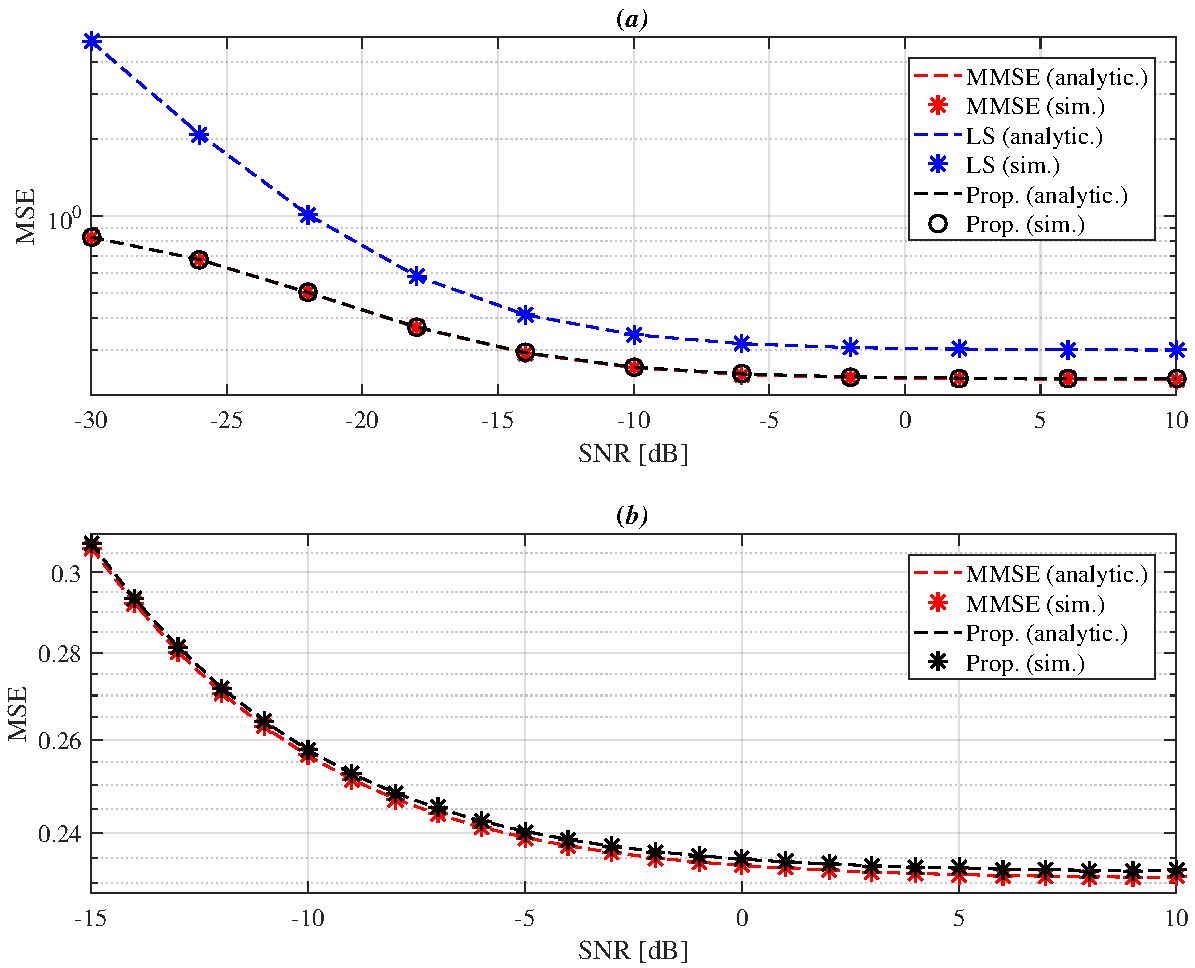
\includegraphics[trim = 0mm 1mm 0mm 0mm, clip=true, scale=0.68]{cropped_mse_vs_snr_for_all_est_ana_and_simu_v1.pdf}
\caption{Channel Estimation MSE versus uplink pilot power.}
\label{fig:snr_vs_mse}
\end{figure}
%------------------------------------------------------------------------------

In Fig. \ref{fig:snr_vs_mse_vs_avg} we vary the number of elements on the main diagonal of $\lVert \textbf{Z}_{ik} \rVert^{2}$ that are averaged to calculate the proposed estimator. The figure shows that the number of elements taken into account directly affects the performance of the proposed estimator, the greater the number of averaged elements, the smaller the MSE gap between the ideal MMSE and the proposed estimator. The number of elements taken into account for the average can also be thought of as the number of paths, $P$, a multichannel has. The figure clearly shows that the performance of the proposed estimator improves with $P$. Therefore, this result shows that the proposed estimator not only exploits spatial diversity but also takes advantage of the time diversity of the delay spread channel profile, since its performance improves with $P$.

%------------------------------------------------------------------------------
\begin{figure}[t]
\centering
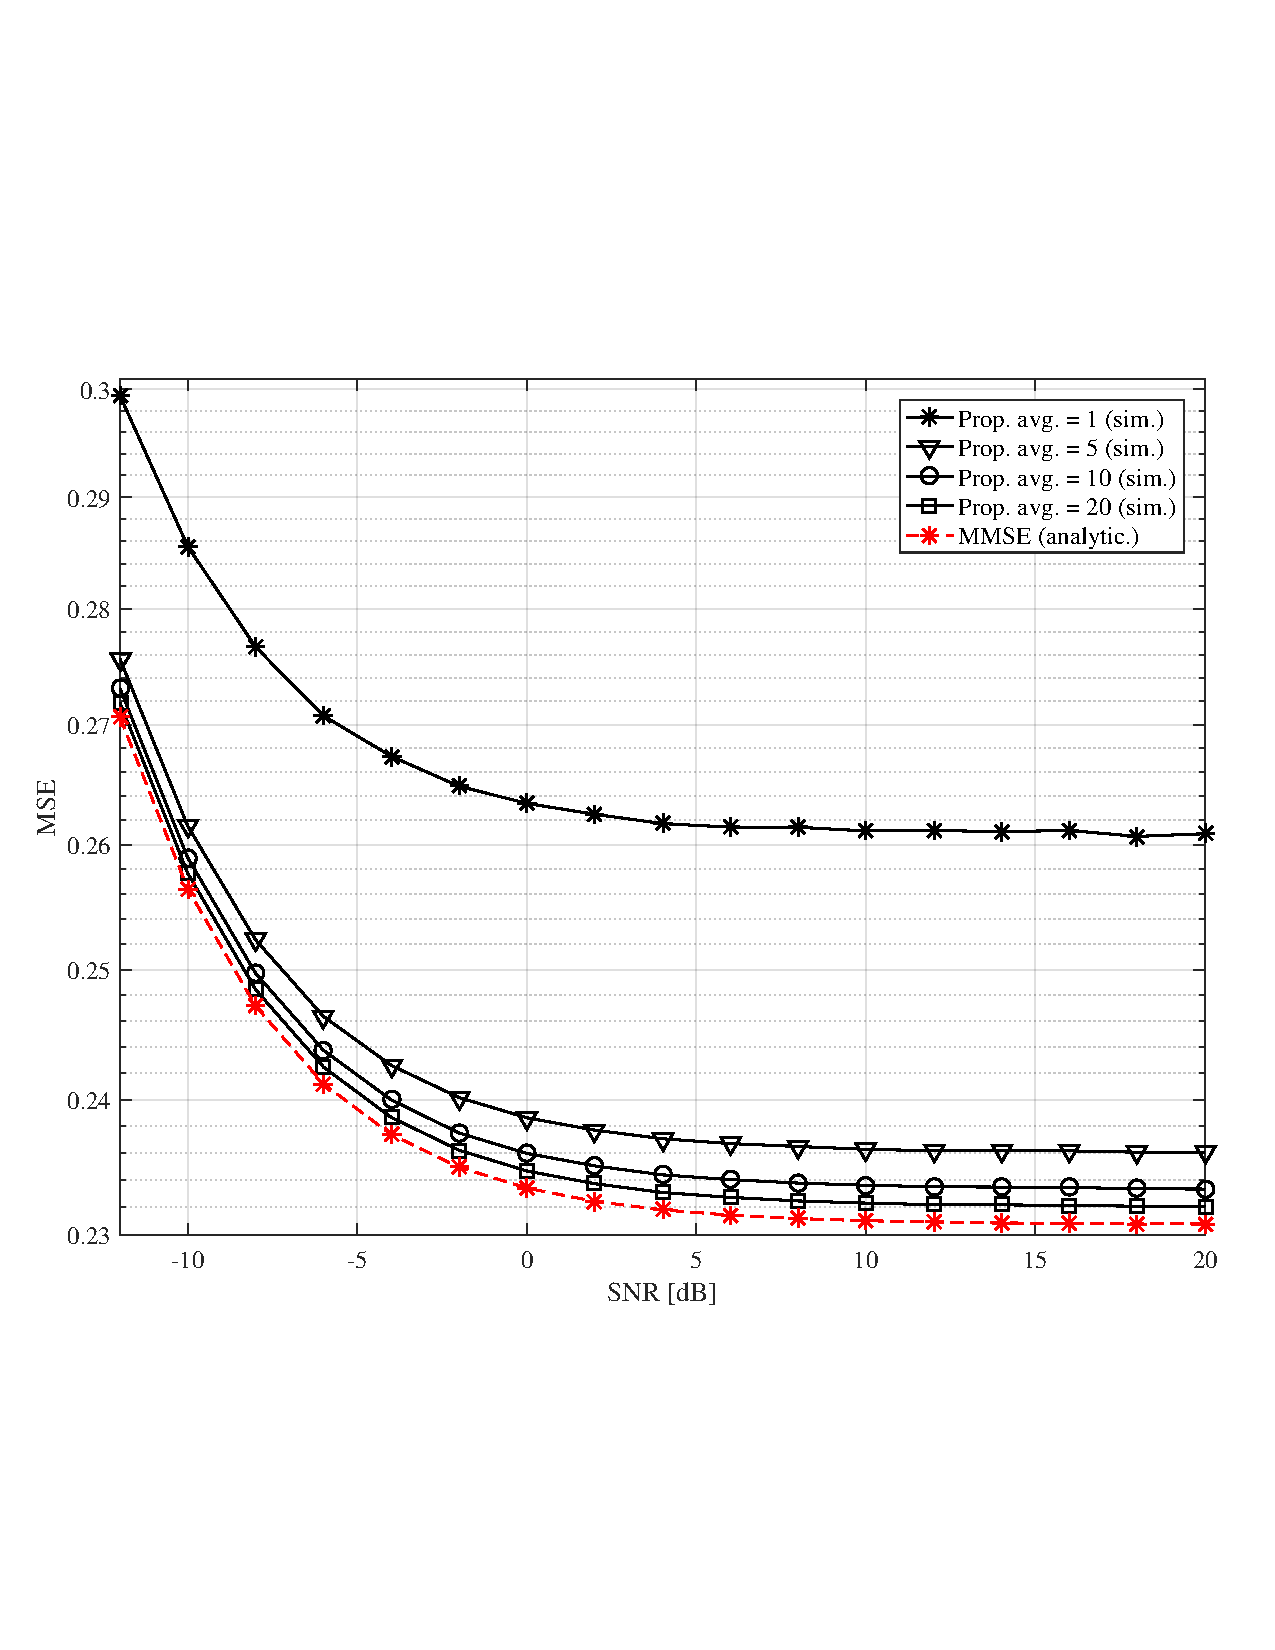
\includegraphics[trim = 0mm 0mm 0mm 0mm, clip=true, scale=0.68]{cropped_mse_vs_snr_vs_p.pdf}
\caption{Impact of the number of averaged elements on the performance of the proposed estimator.}
\label{fig:snr_vs_mse_vs_avg}
\vspace{-4mm}
\end{figure}
%------------------------------------------------------------------------------

%------------------------------------------------------------------------------
\begin{figure}[b]
\vspace{-4mm}
\centering
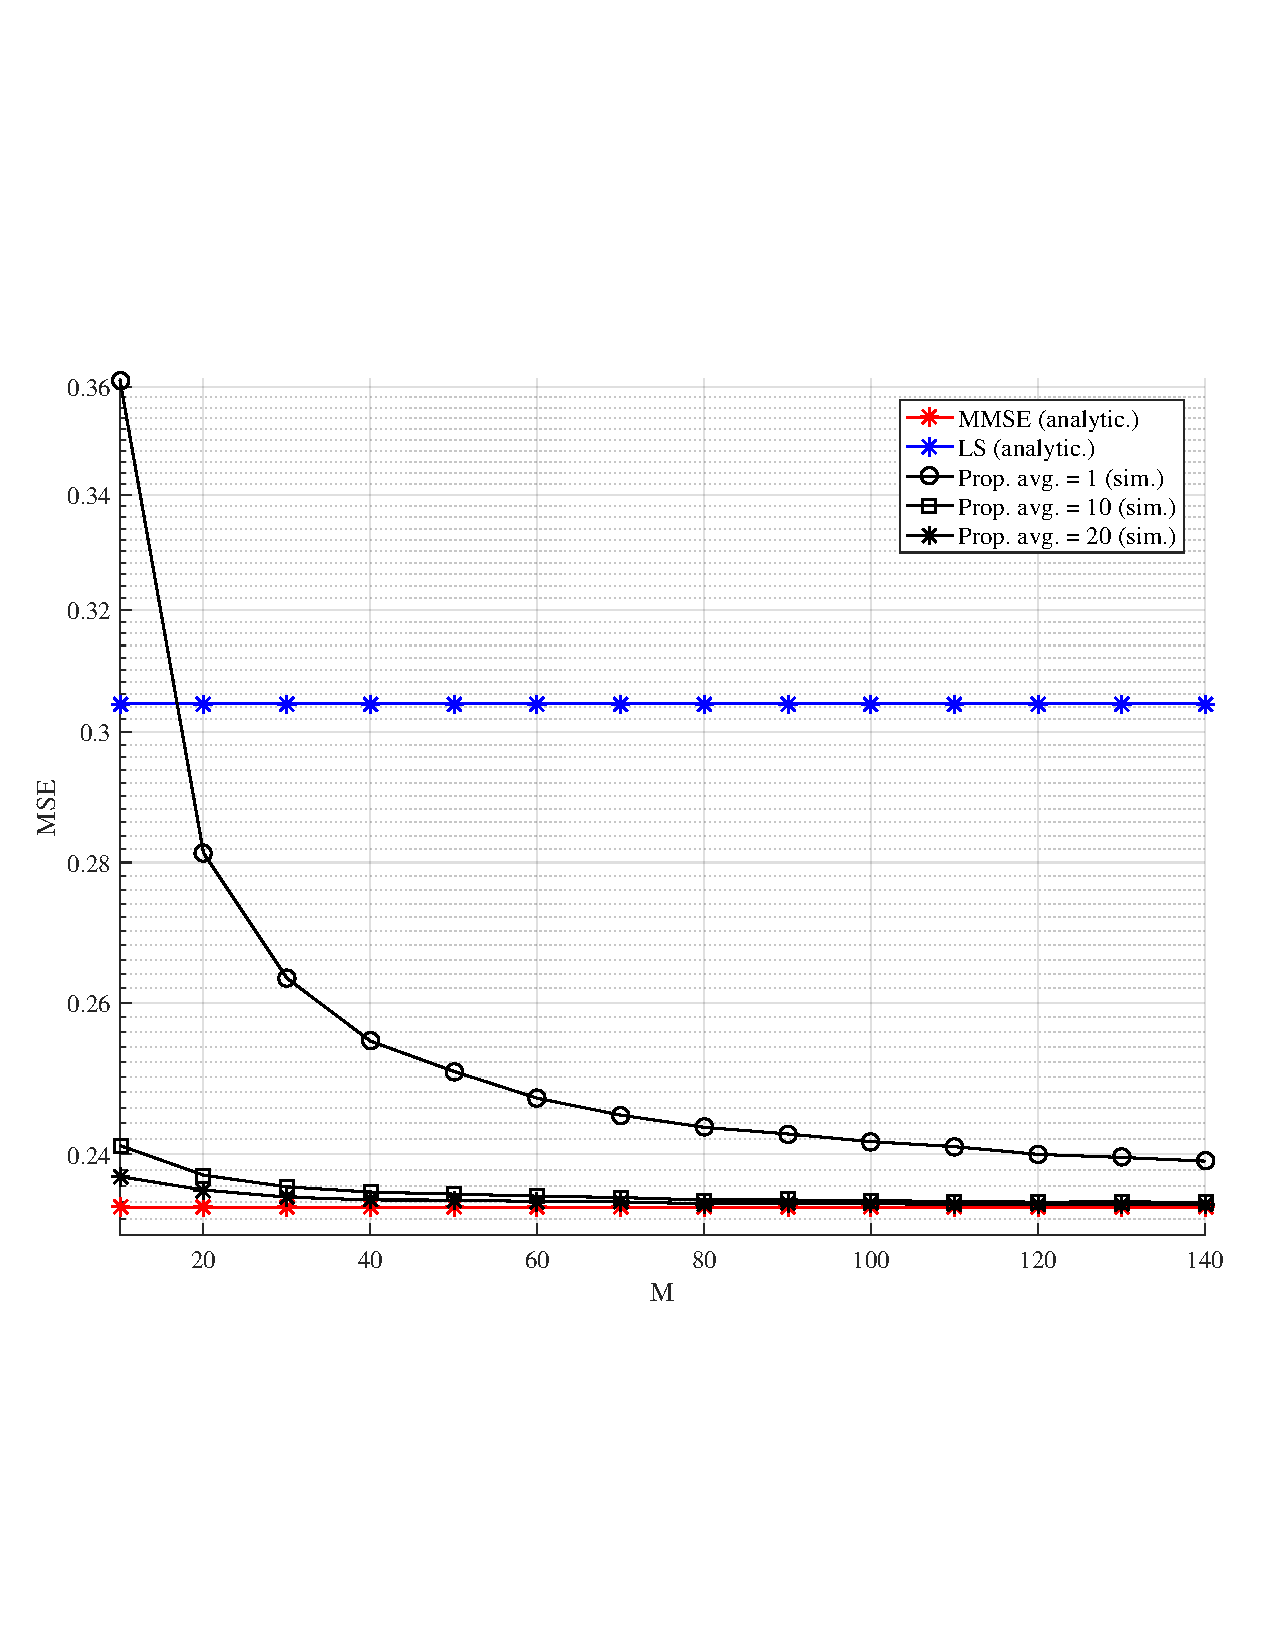
\includegraphics[trim = 0mm 0mm 0mm 1mm, clip=true, scale=0.68]{cropped_mse_vs_m_v1.pdf}
\caption{Channel estimation MSE versus the number of receiving antennas.}
\label{fig:antennas_vs_mse}
\end{figure}
%------------------------------------------------------------------------------

%------------------------------------------------------------------------------
\begin{figure}[t]
\centering
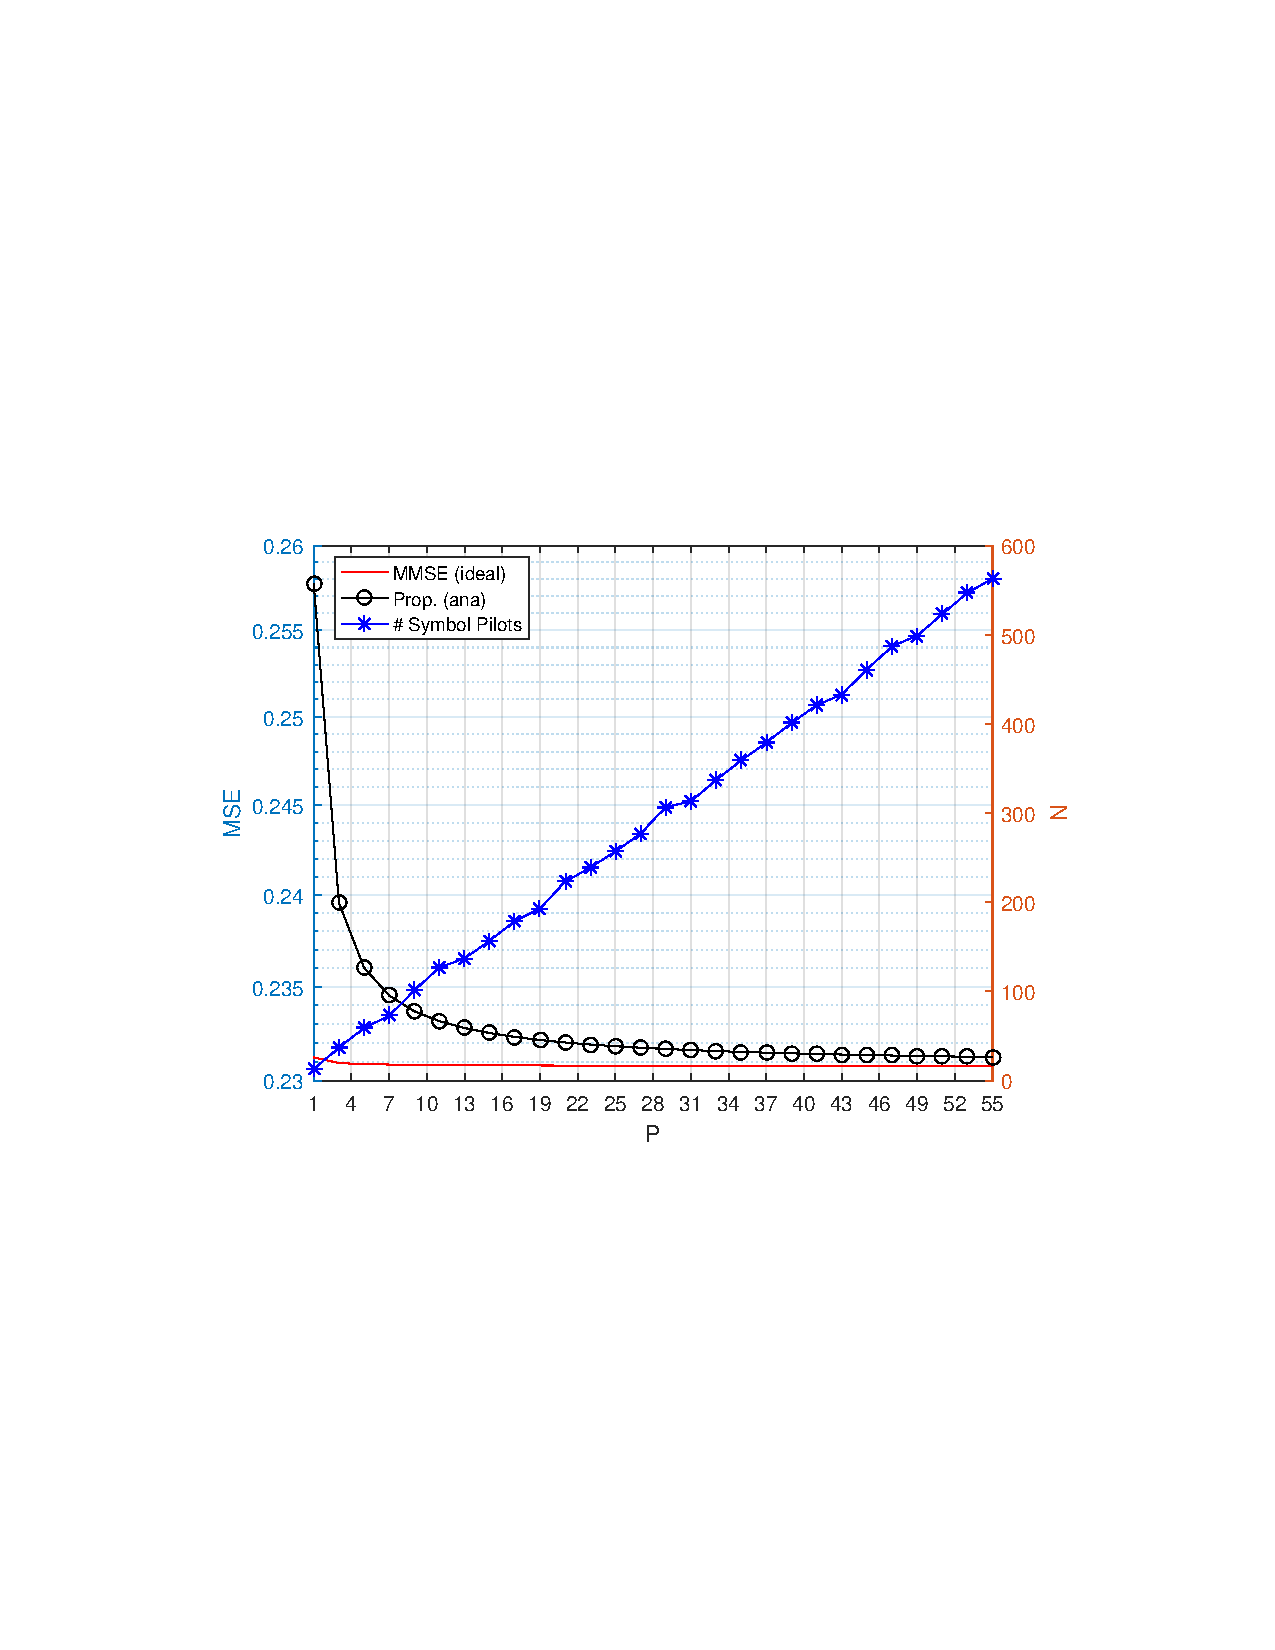
\includegraphics[trim = 0mm 2mm 0mm 1mm, clip=true, scale=0.62]{cropped_mse_vs_p_vs_n_snr20dB_v3.pdf}
\caption{Channel estimation MSE versus the number of channel coefficients versus number of pilot symbols.}
\label{fig:mse_vs_p_vs_n}
\vspace{-4mm}
\end{figure}
%------------------------------------------------------------------------------

%------------------------------------------------------------------------------
\begin{figure}[b]
\vspace{-4mm}
\centering
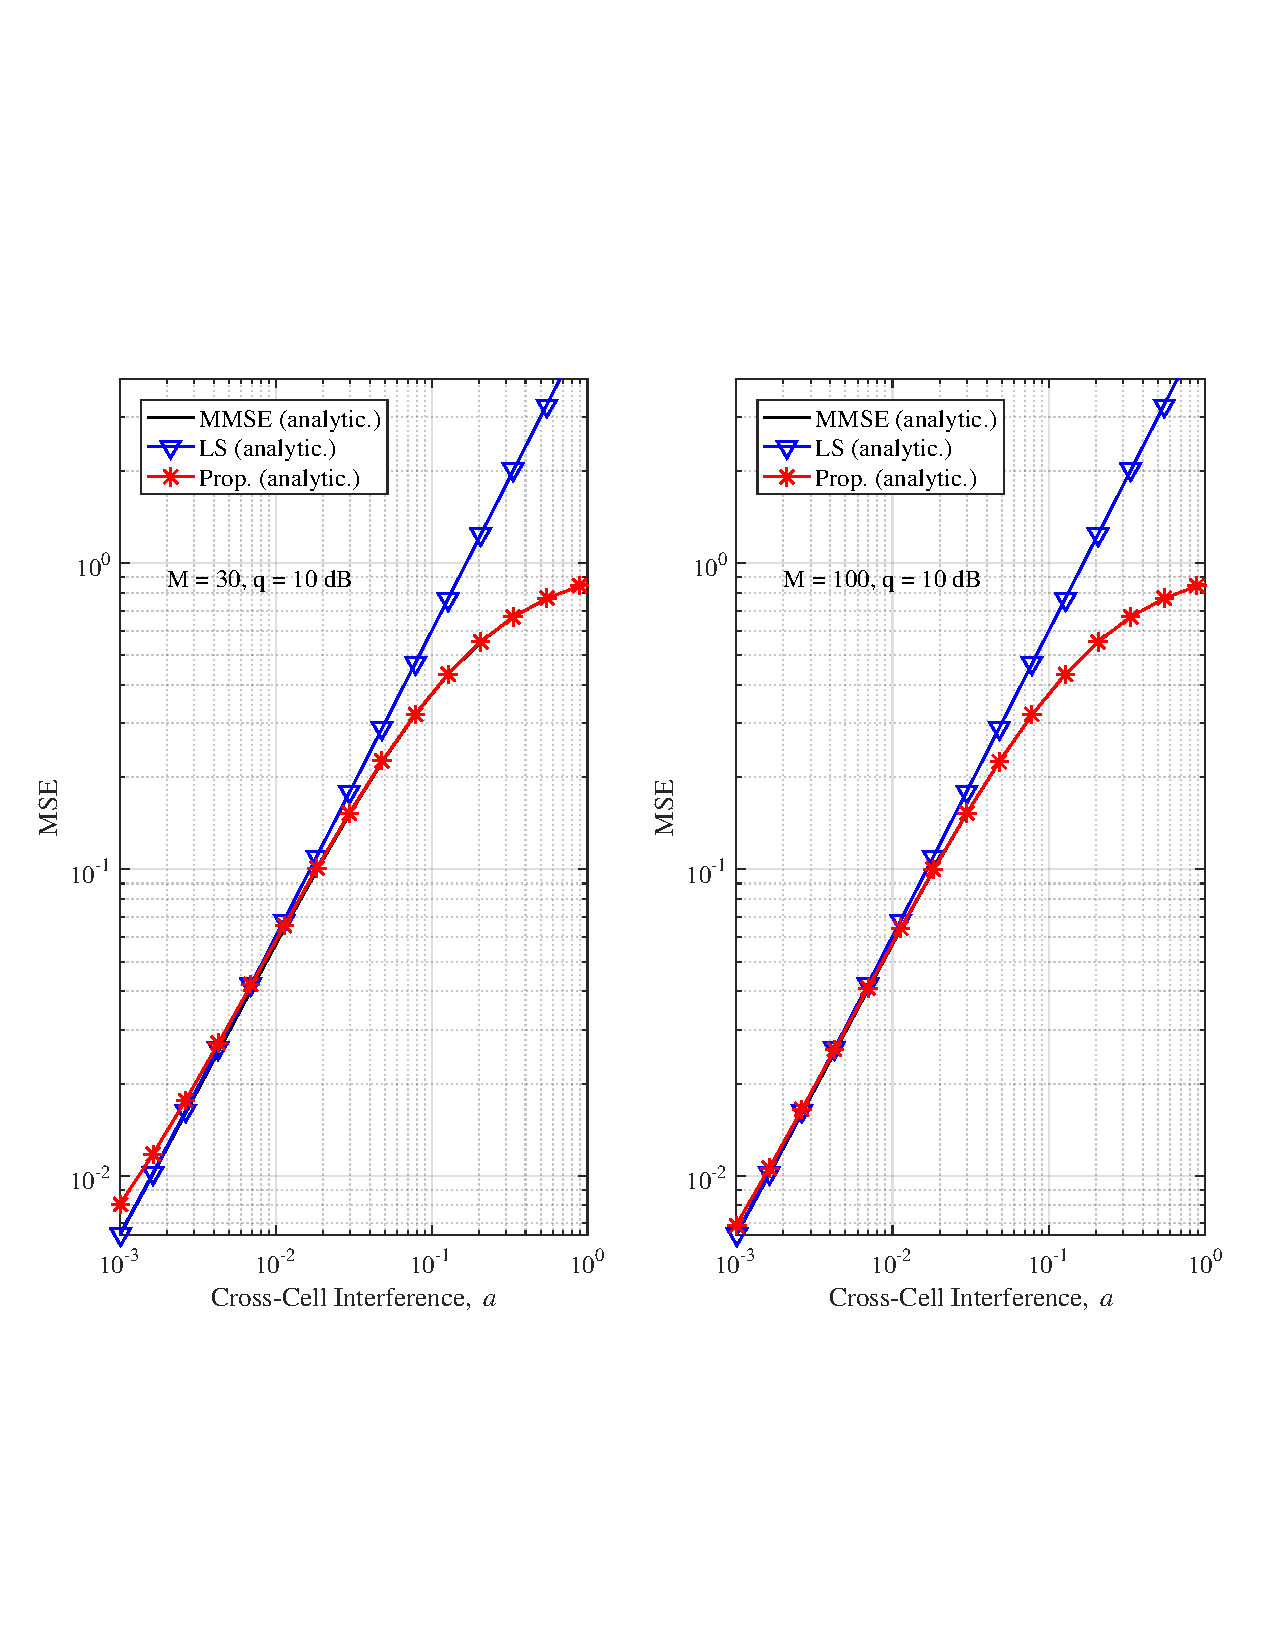
\includegraphics[trim = 0mm 0mm 0mm 0mm, clip=true, scale=0.67]{cropped_mse_vs_a.pdf}
\caption{Channel estimation MSE versus cross-cell interference level.}
\label{fig:mse_vs_a}
\end{figure}
%------------------------------------------------------------------------------

%------------------------------------------------------------------------------
\begin{figure}[t]
\centering
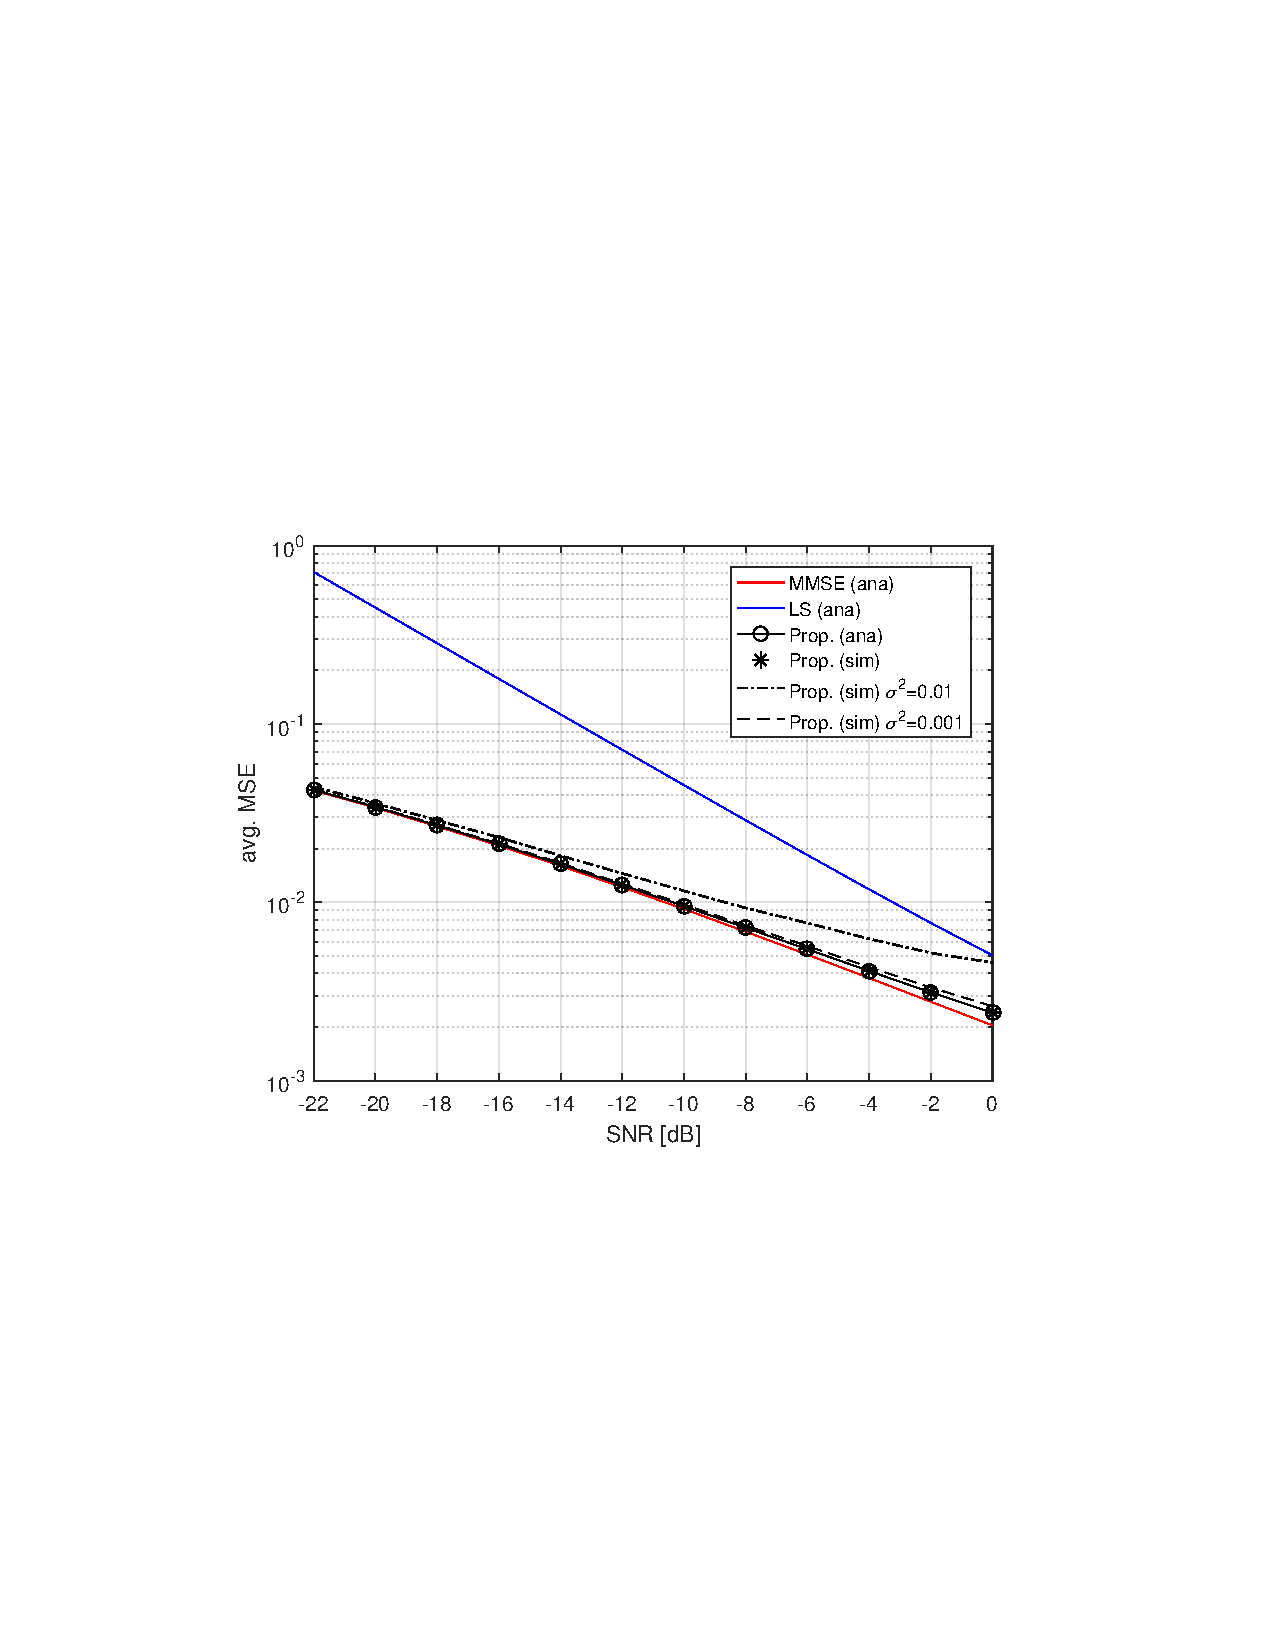
\includegraphics[trim = 0mm 0mm 0mm 0mm, clip=true, scale=0.67]{cropped_snr_vs_avg_mse_random_beta.pdf}
\caption{Average channel estimation MSE under random $\{\beta_{ilk}\}$.}
\label{fig:snr_vs_mse_random_beta}
\vspace{-5mm}
\end{figure}
%------------------------------------------------------------------------------

In Fig. \ref{fig:antennas_vs_mse}, we compare MSE versus the number of BS antennas $M$ under the setting of $a = 0.05$ and TX SNR $q = 0$ dB. With the increase of $M$, the MSE of the proposed estimator approaches that of the ideal MMSE, while the MSE of LS estimator does not change. We also compare the influence of the number of elements of $\lVert \textbf{Z}_{ik} \rVert^{2}$ taken in the average.

In Fig. \ref{fig:mse_vs_p_vs_n}, we compare MSE versus the number of channel coefficients, $P$, versus the pilot symbols length, $N$, for TX SNR $q = 20$ dB and $M = 30$. With the increase of $P$, both the MSE of the proposed method approaches that of the ideal MSE estimator and the number of pilot symbols increase in order to provide users with orthogonal sequences.

In Fig. \ref{fig:mse_vs_a}, we compare MSE performance with respect to various levels of cross-cell interference, here characterized by $a$, with $q = 10$ dB and two different number of antennas, $M = 30$ and $M = 100$. At a low cross-cell interference level, LS presents a slightly better MSE when compared to the proposed estimator. This difference disappears as $M$ increases, as can be noticed in the plot with $M=10$. As the interference level increases, the proposed method outperforms the LS estimator substantially and approaches the ideal MMSE performance (see Remark 4).

In Fig. \ref{fig:snr_vs_mse_random_beta}, we evaluate the MSE performance under random large-scale fading coefficients $\{\beta_{ilk}\}$ with $M=30$. The results are obtained by averaging MSEs over 10000 realizations of $\{\beta_{ilk}\}$. As can be observed, simulation MSE match with the analytical MSE. Additionally, the sensitivity of the proposed estimator against inaccuracy of $\beta_{iik}$ by using an estimate $\beta_{iik} = \beta_{iik}(1 + \mathcal{N}(0,\sigma^{2}))$ is investigated. The performance degradation for $\sigma^{2} = 0.01$ is noticeable at high SNR but for $\sigma^{2} = 0.001$ it is insignificant. The proposed estimator still outperforms the LS estimator significantly.

%**********************************************Conclusions**********************************************
\section{Conclusions}
%******************************************************************************************************

In this work we have proposed an estimation scheme which uses Zadoff-Chu sequences as pilots for the uplink training phase and have introduced a simple and practical channel estimator for multipath multi-cell massive MIMO TDD systems with pilot contamination. The proposed estimator replaces the combined interference, $i.e.$, the summation of the cross-cell large scale coefficients, plus noise power term in the ideal MMSE estimator with a simple and practical estimate. Also, the proposed estimator presents MSE results that are very close to that of the ideal MMSE estimator without requiring knowledge of noise and interference statistics. Additionally, we have derived an approximate analytical MSE expression for the proposed estimator which can be useful in system design and performance evaluation. We have also shown that the MSE expression presented here asymptotically approaches that of the MMSE estimator. Finally, when $P = 1$, the simpler approximate analytical MSE expression presented here can be used instead of the more complex one presented in \cite{Amin:channelEstPilotCont}. 

%**********************************************Appendices**********************************************
\appendices
%-------------------------------------------- Appendix A ---------------------------------------------
\section{}

For the proof of the approximate MSE of the proposed estimator we need to present a few Lemmas and define some matrices.

%************************************************ LEMMA 1 *************************************************
\begin{lemma} If $W \sim \mathcal{CN}(0,\sigma^2)$ then $\lVert W \rVert^{2} \sim \Gamma(1,\sigma^2)$.
\end{lemma}

\begin{IEEEproof} We know that $W = X + jY$ and consequently $\lVert W \rVert^{2} = X^2 + Y^2$, where $X, Y$ are i.i.d. random variables with distribution $\mathcal{N}(0,\sigma^{2}/2)$. Now, if we make $Z = X^2 + Y^2$, then using the joint pdf of $X$ and $Y$ we have that $\mathbb{P}(Z\leq z)$ is defined by
%---------------------------------------------------------------------------------------------
\begin{equation}\label{eq:exponential_into_gamma1}
\mathbb{P}(X^2+Y^2\leq z)= \frac{1}{\pi \sigma^2}\int_{x^2+y^2\leq z}e^{-\frac{(x^2+y^2)}{\sigma^2}} \ dxdy.
\end{equation}
%---------------------------------------------------------------------------------------------

Next, switching to polar coordinates we get:
%---------------------------------------------------------------------------------------------
\begin{equation}\label{eq:exponential_into_gamma2}
\mathbb{P}(Z\leq z) = \frac{1}{\pi \sigma^2}\int_{0}^{2\pi}\int_0^{\sqrt{z}}re^{-\frac{r^2}{\sigma^2}}drd\theta =\frac{2}{\sigma^2}\int_0^{\sqrt{z}}re^{-\frac{r^2}{\sigma^2}}dr.
\end{equation}
%---------------------------------------------------------------------------------------------

Now if we set $u=r^2$ then we get
%---------------------------------------------------------------------------------------------
\begin{equation}\label{eq:exponential_into_gamma3}
\mathbb{P}(Z\leq z)=\frac{1}{\sigma^2}\int_0^ze^{-\frac{u}{\sigma^2}}du,
\end{equation}
%---------------------------------------------------------------------------------------------
so $Z$ is exponentially distributed with rate parameter $\lambda = 1$.

Finally, comparing the pdf given above with the Gamma distribution pdf one can notice that  if the shape parameter $k$ is set to 1 and scale parameter $\theta$ is set to $\sigma^2$ it becomes the exponential pdf, concluding the proof.
\end{IEEEproof}
%********************************************************************************************************

%************************************************ LEMMA 2 *************************************************
\begin{lemma} If $X_{m} \sim \mathcal{CN}(0,\sigma^2) \ \forall m$ are independent, then $\sum_{m=1}^{M}{\lVert X_{m} \rVert^{2}} \sim \Gamma(M,\sigma^2)$.
\end{lemma}
\begin{IEEEproof} From $Lemma$ 1 we know that each $Z_{m} = \lVert X_{m} \rVert^{2} \sim \Gamma(1,\sigma^{2})$. We also know that $Z_{m}$ is independent for all $m$. Therefore, each $Z_{m}$ has the following characteristic function:
%---------------------------------------------------------------------------------------------
\begin{equation}\label{eq:sum_of_gammas1}
\varphi_{Z}(t) = (1-j\sigma^{2}t)^{-1}.
\end{equation}
%---------------------------------------------------------------------------------------------

Next, knowing that the characteristic function of the sum of independent random variables is the product of their individual characteristic functions leads to
%---------------------------------------------------------------------------------------------
\begin{equation}\label{eq:sum_of_gammas2}
\varphi_{Z_{1}+Z_{2}+ ... +Z_{M}}(t) = \varphi_{Z_{1}}(t) \varphi_{Z_{2}}(t) ... \varphi_{Z_{M}}(t) = (1-j\sigma^{2}t)^{-M}.
\end{equation}
%---------------------------------------------------------------------------------------------

Eq. \eqref{eq:sum_of_gammas2} defines the characteristic function of a Gamma-distributed random variable with scale parameter $\theta = \sigma^2$ and shape parameter $k = M$, and therefore concluding the proof.
\end{IEEEproof}
%********************************************************************************************************

%************************************************ LEMMA 3 *************************************************
\begin{lemma} If $X \sim \Gamma(k_1, \theta)$ and $Y \sim \Gamma(k_2, \theta)$ are independent, then $U = \frac{X}{X+Y} \sim \beta(k_1,k_2)$, $V = X + Y \sim \Gamma(k_{1} + k_{2}, \theta)$ and $U$ and $V$ are independent.
\end{lemma}
\begin{IEEEproof} To prove this, first we write the joint pdf of $X$ ans $Y$ as
%-----------------------------------------------------------------------------------------
\begin{equation}\label{eq:lemma3_1}
f_{XY}(x,y) = \frac{\theta^{k_1+ k_2}}{\Gamma(k_1) \Gamma(k_2)} x^{k_1 - 1} \ y^{k_2 - 1} \ e^{-\theta(x+y)}.
\end{equation}
%-----------------------------------------------------------------------------------------

Next, taking the Jacobian determinant of the transformation $X = UV$ and $Y = V(1-U)$ results in
\begin{equation}\label{eq:lemma3_2}
 \left| J \right| = \left| \frac{\partial(x,y)}{\partial(u,v)} \right| = \left| \begin{array}{cc}
\frac{\partial x}{\partial u} & \frac{\partial x}{\partial v} \\
\frac{\partial y}{\partial u} & \frac{\partial y}{\partial v} \end{array} \right| = \left| \begin{array}{cc}
v & u \\
-v & 1-u \end{array} \right| = v.
\end{equation}
%-----------------------------------------------------------------------------------------

Therefore, the joint distribution of $U$ and $V$ has the pdf given by
%-----------------------------------------------------------------------------------------
\begin{equation}\label{eq:lemma3_3}
\begin{split}
f_{UV}(u,v) = f_{XY}(x,y) \left| \frac{\partial(x,y)}{\partial(u,v)} \right| \\ = \frac{\theta^{k_1+ k_2}}{\Gamma(k_1) \Gamma(k_2)} (uv)^{k_1 - 1} \ \left[ v(1-u)\right]^{k_2 - 1} \ e^{-\theta(v)}v \\ = \left\lbrace \frac{\theta^{(k_1 + k_2)}}{\Gamma(k_1 + k_2)} v^{k_1 + k_2 - 1} e^{-\theta v} \right\rbrace  \left\lbrace \frac{u^{k_1 - 1} (1-u)^{k_2 - 1}}{\beta(k_1,k_2)} \right\rbrace,
\end{split}
\end{equation}
%-----------------------------------------------------------------------------------------
and hence, as is apparent from the two terms separated by the curly brackets, $U$ and $V$ are independent random variables with $V \sim \Gamma(k_1 + k_2, \theta)$ and $U \sim \beta(k_1,k_2)$.
\end{IEEEproof}
%********************************************************************************************************

%************************************************ LEMMA 4 *************************************************
\begin{lemma} If $X \sim \Gamma(k,\theta)$ and $\frac{1}{X} \sim \Gamma^{-1}(k,\theta)$, $i.e.$, the Inverse-Gamma distribution, then $\mathbb{E} \left\lbrace \frac{1}{X} \right\rbrace = \frac{1}{\theta(k-1)}$.
\end{lemma}
\begin{IEEEproof} We start this proof by defining the expectation of $Y = \frac{1}{X}$, which is given by
\begin{equation}\label{eq:lemma4_1}
\mathbb{E} \left\lbrace Y \right\rbrace = \int_{0}^{\infty}y \frac{1}{\Gamma(k) \theta^{k}} \left( \frac{1}{y} \right)^{k + 1} e^{-\frac{1}{\theta} \left( \frac{1}{y} \right) } dy.
\end{equation}

Next we apply the following change of variable, $z = \frac{1}{y}$, to \eqref{eq:lemma4_1}, which becomes
\begin{equation}\label{eq:lemma4_2}
\mathbb{E} \left\lbrace Z \right\rbrace =  \frac{1}{\Gamma(k) \theta^{k}} \int_{0}^{\infty} z^{k-2}e^{-\frac{1}{\theta} z } dz.
\end{equation}

By using the following identity 
\begin{equation}\label{eq:lemma4_3}
\int_{0}^{\infty} x^{n} e^{-ax^{b}} = \frac{1}{b} a^{-\left( \frac{n+1}{b} \right)} \Gamma \left( \frac{n+1}{b} \right),
\end{equation}
and knowing that $\Gamma(n) = (n-1)!$, equation \eqref{eq:lemma4_2} can be rewritten as 
\begin{equation}\label{eq:lemma4_4}
\mathbb{E} \left\lbrace Z \right\rbrace = \frac{1}{\Gamma(k) \theta^{k}} \theta^{k-1} \Gamma(k-1) = \frac{1}{\theta (k-1)},
\end{equation}
which concludes the proof.
\end{IEEEproof}
%********************************************************************************************************

%************************************************ LEMMA 5 *************************************************
\begin{lemma} If $X \sim \beta(k_1,k_2)$, $i.e.$, the Beta distribution, then $\mathbb{E}  \left\lbrace X \right\rbrace  = \frac{k_1}{k_1 + k_2}$.
\end{lemma}
\begin{IEEEproof} We start the proof from the definition of the expectation of $X$
\begin{equation}\label{eq:lemma5_1}
\mathbb{E} \left\lbrace X \right\rbrace = \int_{0}^{1} x \frac{1}{\beta(k_1,k_2)} x^{k_{1} - 1 }(1 - x)^{k_{2} - 1} dx.
\end{equation}

By using the following identity 
\begin{equation}\label{eq:lemma5_2}
\beta(\alpha, \beta) = \int_{0}^{1} x^{\alpha -1} (1 - x)^{\beta - 1} dx = \frac{\Gamma(\alpha) \Gamma(\beta)}{ \Gamma(\alpha + \beta)},
\end{equation}
equation \eqref{eq:lemma5_1} can be rewritten as 
\begin{equation}\label{eq:lemma5_3}
\mathbb{E} \left\lbrace X \right\rbrace = \frac{\Gamma(k_1 + k_2)}{ \Gamma(k_1)\Gamma(k_2)}    \frac{\Gamma(k_1 + 1) \Gamma(k_2)}{ \Gamma(k_1 + k_2 + 1)} = \frac{k_1}{k_1 + k_2},
\end{equation}
concluding the proof.
\end{IEEEproof}
%********************************************************************************************************

%************************************************ LEMMA 6 *************************************************
\begin{lemma} Let $\mu_X$ and $\mu_Y$ be the expectations of $X$ and $Y$, $\sigma_{Y}^{2}$ be the variance of $Y$, and $\sigma_{XY}$ be their covariance. Then the expectation, $\mathbb{E} \{X/Y \}$, can be approximated by
%-----------------------------------------------------------------------------------------
\begin{equation}\label{eq:taylor_seriers_expansion}
\mathbb{E} \left\lbrace \frac{X}{Y} \right\rbrace \approx \frac{ \mu_{X} }{ \mu_{Y} } - \frac{\sigma_{XY}}{\mu_{Y}^{2}} + \frac{\mu_{X}}{\mu_{Y}^{3}} \sigma_{Y}^{2}.
\end{equation}
%-----------------------------------------------------------------------------------------
\end{lemma}
\begin{IEEEproof} For a function that depends on two variables, $x$ and $y$, the second order Taylor expansion series about the point $(a,b)$ is given by
%----------------------------------------------------------------------------------
\begin{equation}\label{eq:taylor_seriers_expansion1}
\begin{split}
g(x,y) = g(a,b)+g_{x}(a,b)(x-a) + g_{y}(a,b)(y-b) + \\ +\frac{1}{2!} ( g_{xx}(a,b)(x-a)^2 + 2g_{xy}(a,b)(x-a)(y-b) + \\ + g_{yy}(a,b)(y-b)^{2} ),
\end{split}
\end{equation}
%----------------------------------------------------------------------------------
where the subscripts denote the respective partial derivatives. The partial derivatives are defined by $g_{y} = -X/Y^2$, $g_{yy} = 2X/Y^3$, $g_{x} = 1/Y$, $g_{xx} = 0$, and $g_{xy} = - 1/Y^2$.

Applying the derivatives into \eqref{eq:taylor_seriers_expansion1}, the second order Taylor expansion of $g(X,Y) = X/Y$ around the mean point $(\mu_{X}, \mu_{Y})$ becomes:
%----------------------------------------------------------------------------------
\begin{equation}\label{eq:taylor_seriers_expansion3}
\begin{split}
\frac{X}{Y} \approx \frac{\mu_{x}}{\mu_{y}} - \frac{\mu_{x}}{\mu_{y}^2}(Y - \mu_{y}) + \frac{1}{\mu_{y}}(X - \mu_{x}) \ + \\ +\frac{1}{2!} \left( \frac{2\mu_{x}}{\mu_{y}^3}(Y - \mu_{y})^2 - \frac{2}{\mu_{y}^2}(Y - \mu_{y})(X - \mu_{x}) \right).
\end{split}
\end{equation}
%----------------------------------------------------------------------------------

Finally, applying the expectation operator, $\mathbb{E} \left\lbrace .\right\rbrace$, to \eqref{eq:taylor_seriers_expansion3} concludes the proof.
\end{IEEEproof}
%***************************************************************************************************************************

With the purpose of helping the next proofs, the LS estimator can be expressed the following way
%-----------------------------------------------------------------------------------------
\begin{equation}\label{eq:redefinition_of_z}
\begin{split}
\textbf{Z}_{ik} = \left[\begin{array}{cccc}
\overset{(0)}{{z}_{ik1}} & \overset{(1)}{{z}_{ik1}} & \cdots & \overset{(P-1)}{{z}_{ik1}} \\
\overset{(0)}{{z}_{ik2}} & \overset{(1)}{{z}_{ik2}} & \cdots & \overset{(P-1)}{{z}_{ik2}} \\
\vdots & \vdots & \ddots & \vdots \\
\overset{(0)}{{z}_{ikM}} & \overset{(1)}{{z}_{ikM}} & \cdots & \overset{(P-1)}{{z}_{ikM}} \\ \end{array} \right],
\end{split}
\end{equation}
%-----------------------------------------------------------------------------------------
where $\overset{(p)}{{z}_{ikm}} = \sum_{l=1}^{L} \overset{(p)}{g_{ilkm}} +  \overset{(p)}{w_{ikm}} \sim \mathcal{CN}(0,\zeta_{ik}) \ \forall p$.

With \eqref{eq:redefinition_of_z} the Trace of $\lVert \textbf{Z}_{ik} \rVert^{2}$ can be expressed as
%-----------------------------------------------------------------------------------------
\begin{equation}\label{eq:trace_of_z}
\begin{split}
\Tr ( \lVert \textbf{Z}_{ik} \rVert^{2} ) = \sum_{m=1}^{M} \lVert \overset{(0)}{{z}_{ikm}} \rVert^{2} + \sum_{m=1}^{M} \lVert \overset{(1)}{{z}_{ikm}} \rVert^{2} + \cdots \\ \cdots + \sum_{m=1}^{M} \lVert \overset{(P-1)}{{z}_{ikm}} \rVert^{2} = \sum_{p=0}^{P-1} \sum_{m=1}^{M} \lVert \overset{(p)}{{z}_{ikm}} \rVert^{2}.
\end{split}
\end{equation}
%-----------------------------------------------------------------------------------------

It is important to observe that \eqref{eq:trace_of_z} results in a positive real-valued scalar random variable. From Lemmas 2 and 3 we find that $\Tr ( \lVert \textbf{Z}_{ik} \rVert^{2} ) \sim \Gamma(MP,\zeta_{ik})$.

For the proof of the approximate MSE, we expand $\eta_{ik}^{\text{\text{prop}}} = \frac{1}{M}\mathbb{E}\{ \lVert \hat{\textbf{G}}_{iik}^{\text{prop}} \rVert^{2} \} + \frac{1}{M}\mathbb{E}\{ \lVert \textbf{G}_{iik} \rVert^{2} \} - \frac{2}{M}\mathbb{E} \{\mathfrak{R}\{ (\hat{\textbf{G}}_{iik}^{\text{prop}})^{H} \textbf{G}_{iik} \}\}$ and find these three expected values.

From \eqref{eq:proposed}, \eqref{eq:redefinition_of_z} and \eqref{eq:trace_of_z}, the first expectation can be written as
%----------------------------------------------------------------------------------
\begin{equation}\label{eq:first_term_expectation}
\begin{split}
\frac{1}{M}\mathbb{E}\{ \lVert \hat{\textbf{G}}_{iik}^{\text{prop}} \rVert^{2} \} = M P^{2} \beta_{iik}^{2} \mathbb{E} \left\lbrace \frac{\lVert \textbf{Z}_{ik} \rVert^2}{ [ \Tr ( \lVert \textbf{Z}_{ik} \rVert^{2} ) ]^{2}  } \right\rbrace \\ = a \arraycolsep=1pt\def\arraystretch{1.5} \left[\begin{array}{ccc}
\mathbb{E} \left\lbrace \frac{ X_{ik}^{(0)} }{ \left( \sum_{p=0}^{P-1} X_{ik}^{(p)} \right)^{2} } \right\rbrace & \cdots & \mathbb{E} \left\lbrace \frac{ \sum_{m=1}^{M}{ \overset{*(0)}{{z}_{ikm}} \overset{(P-1)}{{z}_{ikm}} } }{\left( \sum_{p=0}^{P-1} X_{ik}^{(p)} \right)^{2}} \right\rbrace \\
\vdots & \ddots & \vdots \\ 
\mathbb{E} \left\lbrace \frac{ \sum_{m=1}^{M}{ \overset{*(P-1)}{{z}_{ikm}} \overset{(0)}{{z}_{ikm}} } }{\left( \sum_{p=0}^{P-1} X_{ik}^{(p)} \right)^{2}} \right\rbrace & \cdots & \mathbb{E} \left\lbrace \frac{ X_{ik}^{(P-1)} }{\left( \sum_{p=0}^{P-1} X_{ik}^{(p)} \right)^{2}} \right\rbrace  \end{array} \right],
\end{split}
\end{equation}
% \begin{equation}\label{eq:first_term_expectation}
% \begin{split}
% \frac{1}{M}\mathbb{E}\{ \lVert \hat{\textbf{g}}_{iik}^{\text{prop}} \rVert^{2} \} = M P^{2} \beta_{iik}^{2} \mathbb{E} \left\lbrace \frac{\lVert \textbf{z}_{ik} \rVert^2}{ [ \Tr ( \lVert \textbf{z}_{ik} \rVert^{2} ) ]^{2}  } \right\rbrace \\ = a \arraycolsep=-1pt\def\arraystretch{1.5} \left[\begin{array}{ccc}
% \mathbb{E} \left\lbrace \dfrac{ \sum_{m=1}^{M}{\lVert \overset{(0)}{{z}_{ikm}} \rVert^{2} } }{ \left( \sum_{p=0}^{P-1} X_{ik}^{(p)} \right)^{2} } \right\rbrace & \cdots & \mathbb{E} \left\lbrace \dfrac{ \sum_{m=1}^{M}{ \overset{*(0)}{{z}_{ikm}} \overset{(P-1)}{{z}_{ikm}} } }{\left( \sum_{p=0}^{P-1} X_{ik}^{(p)} \right)^{2}} \right\rbrace \\
% \vdots & \ddots & \vdots \\ 
% \mathbb{E} \left\lbrace \dfrac{ \sum_{m=1}^{M}{ \overset{*(P-1)}{{z}_{ikm}} \overset{(0)}{{z}_{ikm}} } }{\left( \sum_{p=0}^{P-1} X_{ik}^{(p)} \right)^{2}} \right\rbrace & \ \cdots \ & \mathbb{E} \left\lbrace \dfrac{ \sum_{m=1}^{M}{\lVert \overset{(P-1)}{{z}_{ikm}} \rVert^{2} } }{\left( \sum_{p=0}^{P-1} X_{ik}^{(p)} \right)^{2}} \right\rbrace  \end{array} \right],
% \end{split}
% \end{equation}
%----------------------------------------------------------------------------------
where $a=M P^{2} \beta_{iik}^{2}$ and $X_{ik}^{(p)} = \sum_{m=1}^{M} \lVert z_{ikm}^{(p)} \rVert^{2} \sim \Gamma(M,\zeta_{ik}) \ \forall p$. Now, we only need to find two types of expectation, one for the terms on the main diagonal and other for the ones on the off-diagonals. 

Firstly, we find the expectation of the terms on the main diagonal of \eqref{eq:first_term_expectation}. From Lemma 3 we know that $U = X_{ik}^{(p)} / \sum_{p=0}^{P-1}{X_{ik}^{(p)}}$ and $V = \sum_{p=0}^{P-1} X_{ik}^{(p)}$ $\forall p$ are independent random variables with $\beta(M,M(P-1))$ and $\Gamma(MP,\zeta_{ik})$ distributions respectively. Also, from the fact that $U$ and $V$ are independent we have that $\mathbb{E} \left\lbrace U/V  \right\rbrace = \mathbb{E} \left\lbrace U  \right\rbrace \mathbb{E} \left\lbrace 1/V  \right\rbrace$, where $1/V \sim \Gamma^{-1}(MP, \zeta_{ik}), $ $i.e.$, the Inverse-Gamma distribution. Lemmas 4 and 5 tell us that $\mathbb{E} \{ 1/V \} = 1 / \zeta_{ik}(MP-1)$ and $\mathbb{E} \{ U \} = 1/P$. Therefore, $a \; \mathbb{E} \{ X_{ik}^{(p)} / ( \sum_{p=0}^{P-1} X_{ik}^{(p)} )^{2} \}  = MP \beta_{iik}^{2} / \zeta_{ik}(MP-1) \ \forall p$. 

Next, we calculate the expectation of the terms on the off-diagonals of \eqref{eq:first_term_expectation}. The ratio of the two random variables, $\sum_{m=1}^{M}{ \overset{*(p)}{{z}_{ikm}} \overset{(p')}{{z}_{ikm}} } \ \forall p \neq p'$ and $( \sum_{p=0}^{P-1} X_{ik}^{(p)} )^{2}$,  does not have a well-defined expectation, $i.e.$ there is no closed formula. However, it is possible to approximate the moments of a function $g(X,Y)$ using Taylor series expansions, provided $g$ is sufficiently differentiable and that the moments of $X$ and $Y$ are finite. Therefore, using Lemma 6 we have that $\mathbb{E} \{ \sum_{m=1}^{M}{ \overset{*(p)}{{z}_{ikm}} \overset{(p')}{{z}_{ikm}} } / (\sum_{p=0}^{P-1}{X_{ik}^{(p)}})^{2} \} \approx 0 \ \forall p \neq p'$. This result was confirmed through simulation. Consequently, the first expectation is given by
%----------------------------------------------------------------------------------
\begin{equation}\label{eq:first_term_expectation2}
\frac{1}{M} \mathbb{E} \left\lbrace \lVert \hat{\textbf{G}}_{iik}^{\text{prop}} \rVert^{2} \right\rbrace = \left[ \frac{MP \beta_{iik}^{2}}{\zeta_{ik}(MP-1)} \right] \textbf{I}_{P}.
\end{equation}
%----------------------------------------------------------------------------------

The second expectation can be written as
%----------------------------------------------------------------------------------
\begin{equation}\label{eq:second_term_expectation}
\begin{split}
\frac{1}{M} \mathbb{E}\{ \lVert \textbf{G}_{iik} \rVert^{2} \} \\ = \arraycolsep=1pt\def\arraystretch{1.5} \left[\begin{array}{ccc} \frac{\sum_{m=1}^{M} \mathbb{E} \{ \lVert g_{iikm}^{(0)} \rVert^{2} \}}{M} & \cdots & \frac{\sum_{m=1}^{M} \mathbb{E} \{ g_{iikm}^{\star (0)}g_{iikm}^{(P-1)} \}}{M} \\
\vdots & \ddots & \vdots \\
\frac{\sum_{m=1}^{M} \mathbb{E} \{ g_{iikm}^{\star(P-1)}g_{iikm}^{(0)} \} }{M} & \cdots & \frac{\sum_{m=1}^{M} \mathbb{E} \{ \lVert g_{iikm}^{(P-1)} \rVert^{2} \} }{M}
\end{array} \right] \\ 
= \left[\begin{array}{ccc} \beta_{iik} & \cdots & 0 \\
\vdots & \ddots & \vdots \\
0 & \cdots & \beta_{iik}
\end{array} \right] = \beta_{iik} \textbf{I}_{P},
\end{split}
\end{equation}
%----------------------------------------------------------------------------------
where the terms, $\sum_{m=1}^{M} \lVert g_{iikm}^{(p)} \rVert^{2} \ \forall p$, in the main diagonal of $\lVert \textbf{G}_{iik} \rVert^{2}$ have Gamma distribution, $\Gamma(M,\beta_{iik})$.

Finally, in order to find the expected value of the third term, first we use \eqref{eq:ls_estimator} and \eqref{eq:proposed} to rewrite it as
%----------------------------------------------------------------------------------
\begin{equation}\label{eq:third_term_expectation}
\begin{split}
-\frac{2}{M}\mathbb{E} \{\mathfrak{R}\{ (\hat{\textbf{G}}_{iik}^{\text{prop}})^{H} \textbf{G}_{iik} \}\} =  -2P \beta_{iik} \mathbb{E} \left\lbrace \mathfrak{R} \left[ \frac{\textbf{Z}_{ik}^{H} \textbf{G}_{iik} }{\Tr \left( \lVert \textbf{Z}_{ik} \rVert^{2} \right)}  \right] \right\rbrace \\
= -2P \beta_{iik} \left\lbrace \mathbb{E} \left[ \frac{\sum_{l=1}^{L} \textbf{G}_{ilk}^{H} \textbf{G}_{iik}}{\Tr \left( \lVert \textbf{Z}_{ik} \rVert^{2} \right)} \right] + \mathbb{E} \left[ \frac{\textbf{W}_{ik}^{H} \textbf{G}_{iik}}{\Tr \left( \lVert \textbf{Z}_{ik} \rVert^{2} \right)} \right] \right\rbrace,
\end{split}
\end{equation}
%----------------------------------------------------------------------------------
where $\textbf{W}_{ik} = \frac{\textbf{N}_{i}\textbf{S}_{k}}{\sqrt{q}N} \sim \mathcal{CN}(\textbf{0}_{M \times P},\frac{M}{qN}\textbf{I}_{P})$. Next, we expand the first expectation term in \eqref{eq:third_term_expectation} as
%----------------------------------------------------------------------------------
\begin{equation}\label{eq:third_term_expectation_1}
\begin{split}
\mathbb{E} \left[ \frac{\sum_{l=1}^{L} \textbf{G}_{ilk}^{H} \textbf{G}_{iik}}{\Tr \left( \lVert \textbf{Z}_{ik} \rVert^{2} \right)} \right] = \left\lbrace \mathbb{E} \left[ \frac{ \textbf{G}_{i1k}^{H} \textbf{G}_{iik}}{\Tr \left( \lVert \textbf{Z}_{ik} \rVert^{2} \right)} \right] +  \right. \\ \left.  \ldots + \mathbb{E} \left[ \frac{ \lVert \textbf{G}_{iik} \rVert^{2} } {\Tr \left( \lVert \textbf{Z}_{ik} \rVert^{2} \right)} \right] + \ldots + \mathbb{E} \left[ \frac{ \textbf{G}_{iLk}^{H} \textbf{G}_{iik}}{\Tr \left( \lVert \textbf{Z}_{ik} \rVert^{2} \right)} \right]  \right\rbrace.
\end{split}
\end{equation}
%----------------------------------------------------------------------------------

Each one of the $L$ expectation terms in \eqref{eq:third_term_expectation_1} can be expressed as
%----------------------------------------------------------------------------------
\begin{equation}\label{eq:second_term_expectation_2}
\begin{split}
\mathbb{E} \left[ \frac{ \textbf{G}_{ilk}^{H} \textbf{G}_{iik}}{\Tr \left( \lVert \textbf{Z}_{ik} \rVert^{2} \right)} \right] \\ = 
\arraycolsep=1pt\def\arraystretch{1.5}
\left[\begin{array}{ccc} \mathbb{E} \left\lbrace \frac{\sum_{m=1}^{M} g_{ilkm}^{\star (0)} g_{iikm}^{(0)} }{\Tr \left( \lVert \textbf{z}_{ik} \rVert^{2} \right)} \right\rbrace & \cdots & \mathbb{E} \left\lbrace \frac{\sum_{m=1}^{M} g_{ilkm}^{\star (0)}g_{iikm}^{(P-1)} }{\Tr \left( \lVert \textbf{z}_{ik} \rVert^{2} \right)} \right\rbrace \\
\vdots & \ddots & \vdots \\
\mathbb{E} \left\lbrace \frac{\sum_{m=1}^{M} g_{ilkm}^{\star(P-1)}g_{iikm}^{(0)} }{\Tr \left( \lVert \textbf{z}_{ik} \rVert^{2} \right)}\right\rbrace & \cdots & \mathbb{E} \left\lbrace \frac{\sum_{m=1}^{M} g_{ilkm}^{\star (P-1)}g_{iikm}^{(P-1)} }{\Tr \left( \lVert \textbf{z}_{ik} \rVert^{2} \right)} \right\rbrace
\end{array} \right].
\end{split}
\end{equation}
%----------------------------------------------------------------------------------

Applying Lemma 6 to the elements on the off-diagonal in \eqref{eq:second_term_expectation_2} we find out that their approximate values are all equal to 0 $\forall l$. Next, applying the same Lemma 6 to the elements on the main diagonal we learn that the L expectation terms in \eqref{eq:third_term_expectation_1} can be approximated as
%----------------------------------------------------------------------------------
\begin{equation}\label{eq:second_term_expectation_3}
\begin{split}
\mathbb{E} \left[ \frac{ \textbf{G}_{ilk}^{H} \textbf{G}_{iik}}{\Tr \left( \lVert \textbf{Z}_{ik} \rVert^{2} \right)} \right] \\ \approx \left\{
\def\arraystretch{1.7}
%\arraycolsep=2pt\def\arraystretch{1.7}
%\renewcommand{\arraystretch}{0.5} % Default value: 1
\begin{array}{cc}
\left[ \frac{M\beta_{iik}(MP+1) \zeta_{ik}}{(MP \zeta_{ik})^{2}} - \frac{M \beta_{iik}^{2}}{(MP \zeta_{ik})^{2}} \right] \textbf{I}_{P},  & l = i\\
\left[-\frac{M \beta_{ilk} \beta_{iik}}{(MP \zeta_{ik})^{2}} \right] \textbf{I}_{P}, & \forall l \neq i.
\end{array}\right.
\end{split}
\end{equation}
%----------------------------------------------------------------------------------

Substituting the results from \eqref{eq:second_term_expectation_3} in \eqref{eq:third_term_expectation_1} we can express it as
%----------------------------------------------------------------------------------
\begin{equation}\label{eq:second_term_expectation_6}
\begin{split}
\mathbb{E} \left[ \frac{\sum_{l=1}^{L} \textbf{G}_{ilk}^{H} \textbf{G}_{iik}}{\Tr \left( \lVert \textbf{Z}_{ik} \rVert^{2} \right)} \right] \\ \approx \frac{M \beta_{iik}}{(MP \zeta_{ik})^{2}} \left[ (MP-1) \zeta_{ik} - \sum_{l=1}^{L}{\beta_{ilk}} \right] \textbf{I}_{P}.
\end{split}
\end{equation}
%----------------------------------------------------------------------------------

The second expectation term in \eqref{eq:third_term_expectation} can be expressed as
%----------------------------------------------------------------------------------
\begin{equation}\label{eq:second_term_expectation_4}
\begin{split}
\mathbb{E} \left[ \frac{\textbf{W}_{ik}^{H} \textbf{G}_{iik}}{\Tr \left( \lVert \textbf{Z}_{ik} \rVert^{2} \right)} \right] \\ = \arraycolsep=0.8pt\def\arraystretch{1.5}
\left[\begin{array}{ccc} \mathbb{E} \left\lbrace \frac{\sum_{m=1}^{M} w_{ikm}^{\star (0)} g_{iikm}^{(0)} }{\Tr \left( \lVert \textbf{z}_{ik} \rVert^{2} \right)} \right\rbrace & \cdots & \mathbb{E} \left\lbrace \frac{\sum_{m=1}^{M} w_{ikm}^{\star (0)}g_{iikm}^{(P-1)} }{\Tr \left( \lVert \textbf{z}_{ik} \rVert^{2} \right)} \right\rbrace \\
\vdots & \ddots & \vdots \\
\mathbb{E} \left\lbrace \frac{\sum_{m=1}^{M} w_{ikm}^{\star(P-1)}g_{iikm}^{(0)} }{\Tr \left( \lVert \textbf{z}_{ik} \rVert^{2} \right)}\right\rbrace & \cdots & \mathbb{E} \left\lbrace \frac{\sum_{m=1}^{M} w_{ikm}^{\star (P-1)}g_{iikm}^{(P-1)} }{\Tr \left( \lVert \textbf{z}_{ik} \rVert^{2} \right)} \right\rbrace
\end{array} \right].
\end{split}
\end{equation}
%----------------------------------------------------------------------------------

Now, applying Lemma 6 to the off-diagonal terms in \eqref{eq:second_term_expectation_4} we also find out that their approximate values are all equal to 0. Therefore, applying Lemma 6 to the elements on the main diagonal we determine that \eqref{eq:second_term_expectation_4} can be approximated as
%----------------------------------------------------------------------------------
\begin{equation}\label{eq:second_term_expectation_5}
\mathbb{E} \left[ \frac{\textbf{W}_{ik}^{H} \textbf{G}_{iik}}{\Tr \left( \lVert \textbf{Z}_{ik} \rVert^{2} \right)} \right] \approx \left[ -\frac{M \beta_{iik} / qN}{(MP \zeta_{ik})^{2}} \right] \textbf{I}_{P}.
\end{equation}
%----------------------------------------------------------------------------------

Substituting the results from \eqref{eq:second_term_expectation_6} and \eqref{eq:second_term_expectation_5} back in \eqref{eq:third_term_expectation} we find the third expectation
%----------------------------------------------------------------------------------
\begin{equation}\label{eq:second_term_expectation_7}
-\frac{2}{M} \mathbb{E} \{\mathfrak{R}\{ (\hat{\textbf{G}}_{iik}^{\text{prop}})^{H} \textbf{G}_{iik} \}\} \approx -\frac{2 \beta_{iik}^{2}}{\zeta_{ik}} \textbf{I}_{P}.
\end{equation}
%----------------------------------------------------------------------------------

After finding the three expectations, \eqref{eq:first_term_expectation2}, \eqref{eq:second_term_expectation} and \eqref{eq:second_term_expectation_7}, by substituting them back in the expansion of $\eta_{ik}^{\text{\text{prop}}}$, we complete the proof.

%-------------------------------------------- Appendix B ---------------------------------------------
\section{}
Here we present proof for \eqref{eq:distance_mmse_prop}. We expand $\frac{1}{M} \mathbb{E} \left\lbrace \lVert \hat{\textbf{G}}_{iik}^{\text{prop}} - \hat{\textbf{G}}_{iik}^{\text{MMSE}} \rVert^{2} \right\rbrace = \frac{1}{M}\mathbb{E}\{ \lVert \hat{\textbf{G}}_{iik}^{\text{prop}} \rVert^{2} \} + \frac{1}{M}\mathbb{E}\{ \lVert \hat{\textbf{G}}_{iik}^{\text{MMSE}} \rVert^{2} \} - \frac{2}{M}\mathbb{E} \{\mathfrak{R}\{ (\hat{\textbf{G}}_{iik}^{\text{prop}})^{H} \hat{\textbf{G}}_{iik}^{\text{MMSE}} \}\}$. Then we compute the different expectations. The first expectation is given by \eqref{eq:first_term_expectation2}, $\frac{1}{M}\mathbb{E}\{ \lVert \hat{\textbf{G}}_{iik}^{\text{prop}} \rVert^{2} \} = \left[ {MP \beta_{iik}^{2}} / {\zeta_{ik}(MP-1)} \right] \textbf{I}_{P}$. Next, by recalling that $\hat{\textbf{G}}_{iik}^{\text{MMSE}} \sim \mathcal{CN}(\textbf{0}_{M \times P}, ({M \beta_{iik}^{2}} / {\zeta_{ik}} )  \textbf{I}_{P})$ we have $\frac{1}{M}\mathbb{E}\{ \lVert \hat{\textbf{G}}_{iik}^{\text{MMSE}} \rVert^{2} \} = ( {\beta_{iik}^{2}}  / {\zeta_{ik}} ) \textbf{I}_{P}$. For the last term, using \eqref{eq:mmse} and \eqref{eq:proposed}, and then \eqref{eq:redefinition_of_z} and \eqref{eq:trace_of_z}, we can write it as
%----------------------------------------------------------------------------------
\begin{equation}\label{eq:appendix_b_1}
\begin{split}
-\frac{2}{M}\mathbb{E} \{\mathfrak{R}\{ (\hat{\textbf{G}}_{iik}^{\text{prop}})^{H} \hat{\textbf{G}}_{iik}^{\text{MMSE}} \}\} = -\frac{2P \beta_{iik}^{2}}{\zeta_{ik}} \mathbb{E} \left\lbrace \frac{\lVert \textbf{Z}_{ik} \rVert^2}{ \Tr ( \lVert \textbf{Z}_{ik} \rVert^{2} ) } \right\rbrace \\ = c \arraycolsep=1pt\def\arraystretch{1.5} \left[\begin{array}{ccc}
\mathbb{E} \left\lbrace \frac{ X_{ik}^{(0)} }{ \sum_{p=0}^{P-1} X_{ik}^{(p)} } \right\rbrace & \cdots & \mathbb{E} \left\lbrace \frac{ \sum_{m=1}^{M}{ \overset{*(0)}{{z}_{ikm}} \overset{(P-1)}{{z}_{ikm}} } }{ \sum_{p=0}^{P-1} X_{ik}^{(p)} } \right\rbrace \\
\vdots & \ddots & \vdots \\ 
\mathbb{E} \left\lbrace \frac{ \sum_{m=1}^{M}{ \overset{*(P-1)}{{z}_{ikm}} \overset{(0)}{{z}_{ikm}} } }{ \sum_{p=0}^{P-1} X_{ik}^{(p)} } \right\rbrace & \cdots & \mathbb{E} \left\lbrace \frac{ X_{ik}^{(P-1)} }{ \sum_{p=0}^{P-1} X_{ik}^{(p)} } \right\rbrace  \end{array} \right],
\end{split}
\end{equation}
%----------------------------------------------------------------------------------
where $c = -{2P \beta_{iik}^{2}} / {\zeta_{ik}}$ and $X_{ik}^{(p)} = \sum_{m=1}^{M} \lVert z_{ikm}^{(p)} \rVert^{2} \ \forall p$. Applying Lemma 3 to the elements on the main diagonal we have that $U = X_{ik}^{(p)} / \sum_{p=0}^{P-1}{X_{ik}^{(p)}} \sim \beta(M,M(P-1)) \ \forall p$ where $\mathbb{E}\{ U \} = 1/P$. Next, applying Lemma 6 to the elements on the off diagonal we have $\mathbb{E} \{ \sum_{m=1}^{M}{ \overset{*(p)}{{z}_{ikm}} \overset{(p')}{{z}_{ikm}} } / \sum_{p=0}^{P-1}{X_{ik}^{(p)}} \} \approx 0 \ \forall p \neq p'$. Therefore, $-\frac{2}{M}\mathbb{E} \{\mathfrak{R}\{ (\hat{\textbf{G}}_{iik}^{\text{prop}})^{H} \hat{\textbf{G}}_{iik}^{\text{MMSE}} \}\} = -({2 \beta_{iik}^{2}} / {\zeta_{ik}}) \textbf{I}_{P}$. Finally, by substituting these quantities back into the expansion, we arrive at \eqref{eq:distance_mmse_prop}.

\begin{thebibliography}{1}

%% ********* Introduction on Massive MIMO *************
\bibitem{marzetta:noncooperative}T. L. Marzetta, \textquotedblleft{Noncooperative cellular wireless with unlimited numbers of base station antennas\textquotedblright}, \emph{IEEE Trans. Wireless Commun.}, vol. 9, no. 11, pp. 3590-3600, Nov. 2010.

\bibitem{larsson:mmimo_next_gen}Erik G. Larsson, Ove Edfors, Fredrik Tufvesson and Thomas L. Marzetta, \textquotedblleft{Massive MIMO for next generation wireless systems\textquotedblright}, \emph{IEEE Commun. Mag.}, vol. 52, no. 2, Feb. 2014.

%% ******* Papers on Pilot Contamination ************
\bibitem{marzetta:pilotContamination}J. Jose, A. Ashikhmin, T. L. Marzetta, and S. Vishwanath, \textquotedblleft{Pilot contamination and precoding in multi-cell TDD systems\textquotedblright},  \emph{IEEE Trans. Wireless Commun.}, vol. 10, no. 8, pp. 2640-2651, Aug. 2011.

\bibitem{emil:10_myths}Emil Bjornson, Erik G. Larsson and Thomas L. Marzetta, \textquotedblleft{Massive MIMO: ten myths and one critical question\textquotedblright}, \emph{IEEE Commun. Mag.}, vol. 54, no. 2, Feb. 2016.

\bibitem{marzetta:book}Thomas L. Marzetta, Erik G. Larsson, Hong Yang and Hien Quoc Ngo, \textquotedblleft{Fundamentals of Massive MIMO\textquotedblright}, Cambridge University Press, Nov. 2016.

%% *********** Channel Estimation (LS) *****************
\bibitem{Gesbert:coordinated}H. Yin, D. Gesbert, M. Filippou and Y. Liu, \textquotedblleft{A Coordinated Approach to Channel Estimation in Large-Scale Multiple Antenna Systems\textquotedblright}, \emph{IEEE Journal on Selected Areas in Communications}, vol. 31, no. 2, pp. 264-273, Feb. 2013.

%% *********** Channel Estimation (MMSE) ***************
\bibitem{Debbah:howmanyantennas}J. Hoydis, S. ten Brink, and M. Debbah, \textquotedblleft{Massive MIMO in the UL/DL of cellular networks: How many antennas do we need?\textquotedblright}, \emph{IEEE J. Sel. Areas Commun.}, vol. 31, no. 2, pp. 160-171, Feb. 2013.

\bibitem{Marzetta:finitedimensionalchannels}H. Q. Ngo, E. G. Larsson, and T. L. Marzetta, \textquotedblleft{The multicell multiuser MIMO uplink with very large antenna arrays and a finite-dimensional channel\textquotedblright}, \emph{IEEE Trans. Commun.}, vol. 61, no. 6, pp. 2350-2361, Jun. 2013.

\bibitem{Ashikhmi:interference_reduction}A. Ashikhmi, T. L. Marzetta, and L. Li, \textquotedblleft{Interference reduction in multi-cell massive MIMO systems I: large-scale fading precoding and decoding\textquotedblright}, arXiv preprint arXiv:1411.4182, 2014.

%% ******* Papers on channel estimation considering only flat channel *******.
\bibitem{khushboo:semi_blind_est}Khushboo Mawatwal, Debarati Sen, and Rajarshi Roy, \textquotedblleft{A Semi-Blind Channel Estimation Algorithm for Massive MIMO Systems\textquotedblright}, \emph{IEEE Wireless Commun. Letters}, vol. 6, no. 1, pp. 70-73, Feb. 2017.

\bibitem{tadashi:asynch_mu_chann_est}Ricardo Tadashi Kobayashi  and Taufik Abrão, \textquotedblleft{Theoretical error for asynchronous multi-user large-scale MIMO channel estimation\textquotedblright}, \emph{IET Communications}, vol. 11, no. 1, pp. 17-24, Dec. 2016.

\bibitem{fang:low_rank}Jun Fang, Xingjian Li, Hongbin Li and Feifei Gao, \textquotedblleft{Low-Rank Covariance-Assisted Downlink Training and Channel Estimation for FDD Massive MIMO Systems\textquotedblright}, \emph{IEEE Trans. on Wireless Commun.}, vol. 16, no. 3, March 2017.

\bibitem{mojtaba:traning_for_decorr_chann_est}Mojtaba Soltanalian, Mohammad Mahdi Naghsh, Nafiseh Shariati, Petre Stoica and Babak Hassibi, \textquotedblleft{Training Signal Design for Correlated Massive MIMO Channel Estimation\textquotedblright}, \emph{IEEE Trans. on Wireless Commun.}, vol. 16, no. 2, Feb. 2017.

\bibitem{Bjornson:LowComplexityPolynomial}N. Shariati, E. Bjornson, M. Bengtsson and M. Debbah, \textquotedblleft{Low-Complexity Polynomial Channel Estimation in Large-Scale MIMO with Arbitrary Statistics\textquotedblright}, \emph{IEEE Journal of Selected Topics in Signal Processing}, vol. 8, no. 5, pp. 815-830, Oct. 2014.

\bibitem{noh:Pilot_beam_pattern}S. Noh, M. D. Zoltowski, Y. Sung, and D. J. Love, \textquotedblleft{Pilot beam pattern design for channel estimation in massive MIMO systems\textquotedblright}, \emph{IEEE Journal of Selected Topics in Signal Processing}, vol. 8, no. 5, pp. 787-801, Oct. 2014.

\bibitem{Truong:Channel_Aging}K. T. Truong and R. W. Heath, \textquotedblleft{Effects of Channel Aging in Massive MIMO Systems\textquotedblright}, \emph{Journal of Communications and Networks}, vol. 15, no. 4, pp. 338-351, August 2013.

\bibitem{Muller:Blind_Decontamination}R. R. Muller, L. Cottatellucci, and M. Vehkapera, \textquotedblleft{Blind Pilot Decontamination\textquotedblright}, \emph{IEEE Journal of Selected Topics in Signal Processing}, vol. 8, no. 5, pp. 773-786, Oct 2014.

\bibitem{Amin:channelEstPilotCont}Amin Khansefid, Hlaing Minn, 
\textquotedblleft{On Channel Estimation for Massive MIMO With Pilot Contamination\textquotedblright}, \emph{IEEE Communications Letters.}, vol. 19, no. 9, pp. 1660-1663, Sept. 2015.

% TDD Protocol.

%\bibitem{emil:comb_vs_multi_stream}E. Bjornson, M. Kountouris, M. Bengtsson, and B. Ottersten, \textquotedblleft{Receive combining vs. multi-stream multiplexing in downlink systems with multi-antenna users\textquotedblright}, \emph{IEEE Trans. Signal Process.}, vol. 61, no. 13, pp. 3431-3446, Jul. 2013.

\bibitem{marzetta:how_much_training}T. L. Marzetta, \textquotedblleft{How much training is required for multiuser MIMO?\textquotedblright}, in \emph{Proc. 40th Asilomar Conf. Signals, Syst., Comput. (ACSSC)}, Pacific Grove, CA, USA, Oct. 2006, pp. 359-363.

\bibitem{caire:achivable_dl_rates}G. Caire, N. Jindal, M. Kobayashi, and N. Ravindran, \textquotedblleft{Multiuser MIMO achievable rates with downlink training and channel state feedback\textquotedblright}, \emph{IEEE Trans. Inf. Theory}, vol. 56, no. 6, pp. 2845-2866, Jun. 2010.

% Mobile Channel: Large and small-scale fading.
\bibitem{rappaport:wireless_comm}T. S. Rappaport, \textquotedblleft{Wireless Communications: Principles and Practice\textquotedblright}, 2nd ed. Singapore: Pearson Education, Inc., 2002.

\bibitem{sklar:rayleigh_channels}Bernard Sklar, \textquotedblleft{Rayleigh Fading Channels in Mobile Digital Communication Systems Part I: Characterization\textquotedblright}, \emph{IEEE Communications Magazine}, vol. 35, no. 7, pp. 90-100, Sept. 1997.

\bibitem{tranter:principles}W. H. Tranter, K. S. Shanmugan, T. S. Rappaport and K. L. Kosbar, \textquotedblleft{Principles of Communication Systems Simulation with Wireless Applications\textquotedblright}, Prentice Hall, 2004, ISBN 0-13-494790-8.

% Zadoff-Chu Sequences.
\bibitem{zadoffchu:zadoffchu}David C. Chu, \textquotedblleft{Polyphase codes with good periodic correlation properties\textquotedblright}, \emph{IEEE Transactions on Information Theory}, pp. 531-532, July 1972.

\bibitem{kay:estimationbook}S. M. Kay, \textquotedblleft{Fundamentals of Statistical Signal Processing, Volume I: Estimation Theory\textquotedblright}, New York, NY, USA: Pearson Education, 1993.

\bibitem{fengChen:largeScale}Ko-Feng Chen, Yen-Cheng Liu, Yu T Su, \textquotedblleft{On composite channel estimation in wireless massive MIMO systems\textquotedblright}, \emph{IEEE Globecom Workshops}, pp 135-139, Sept. 2013.

\end{thebibliography}
 
\end{document}
